This chapter provides an overview of the proof theoretic basis behind LM
and the dynamic semantics of the language. First, we will present the subset of
linear logic from which LM is built on. Second, we present the high level
dynamic semantics - how rules are evaluated and node communication - followed by
the low level dynamics, a close representation of how the virtual machine runs.
Finally, we prove that the low level dynamic semantics are sound in relation to
the high level dynamic semantics.

\section{Linear Logic}

Logic, as \emph{classically} understood, treats true propositions as
\emph{persistent truth}. When a persistent proposition is needed to prove other
propositions, it can be reused as many times as we wish because it is true
indefinitely. This is also true in the \emph{constructive} or
\emph{intuitionistic} school of logic.  Linear logic is a \emph{substructural
logic} (lacks weakening and contraction) developed by
Girard~\cite{Girard95logic:its} extends \emph{persistent logic} with linear
propositions which can be understood as ephemeral resources that can be used
only once to prove other propositions.  Naturally, linear logic is well
suited for modeling computing systems that deal with state, of which LM is
one of them.  Traditional forward-chaining logic programming languages like
Datalog only use persistent logic, however many ad-hoc
extensions~\cite{Liu98extendingdatalog,Ludascher95alogical} have been devised
in to support state updates, but most are extra-logical which makes it harder
to reason about programs. LM uses linear logic as its foundation, therefore
state updates are natural to the language.

In linear logic, truth is treated as a resource that is consumed once used. For
instance, in the graph visit program in Fig.~\ref{code:visit}, the
\texttt{unvisited(A)} and \texttt{visit(A)} linear facts are consumed in order
to prove \texttt{visit(A)} and the comprehension. If those facts were
persistent, then the rule would make no sense, because the node would be
\texttt{visited} and \texttt{unvisited} at the same time!

\subsection{Sequent Calculus}

We now describe the linear logic fragment used as a basis for LM.  Note that in
this thesis we follow the intuitionistic approach and use the sequent
calculus~\cite{gen35} to specify the logic. Our initial sequent is written as
$\Psi; \seqx{\Gamma}{\Delta}{C}$ and can be read as "assuming persistent
resources $\Gamma$ and linear resources $\Delta$ then $C$ is true".  More
specifically, $\Psi$ is the typing context which contains unique variables,
$\Gamma$ is a multi-set of persistent resources, $\Delta$ is a multi-set of
linear resources while $C$ is the proposition we want to prove.

We first have the \emph{simultaneous conjunction} $A \otimes B$ that packages
linear resources together. In the right rule, $A \otimes B$ is true if both $A$
and $B$ are true, and, in the left rule, it is possible to split $A \otimes B$
apart.


\[
\infer[\otimes R]
{\Psi ; \seqx{\Gamma}{\Delta, \Delta'}{A \otimes B}}
{\Psi ; \seqx{\Gamma}{\Delta}{A} & \Psi ; \seqx{\Gamma}{\Delta}{B}}
\tab
\infer[\otimes L]
{\Psi ; \seqx{\Gamma}{\Delta, A \otimes B}{C}}
{\Psi ; \seqx{\Gamma}{\Delta, A, B}{C}}
\]



Next, we have the \emph{additive conjunction} $A \with B$ that allows us to
select between $A$ or $B$. In the right rule we must prove $A$ and $B$ using
the same resources, while in the left rule, we can select one of the
resources.

\[
   \infer[\with L_1]
   {\Psi; \seqx{\Gamma}{\Delta, A \with B}{C}}
   {\Psi; \seqx{\Gamma}{\Delta, A}{C}}
   \tab
   \infer[\with L_2]
   {\Psi; \seqx{\Gamma}{\Delta, A \with B}{C}}
   {\Psi; \seqx{\Gamma}{\Delta, B}{C}}
   \tab
   \infer[\with R]
   {\Psi; \seqx{\Gamma}{\Delta}{A \with B}}
   {\Psi; \seqx{\Gamma}{\Delta}{A} & \Psi; \seqx{\Gamma}{\Delta}{B}}
\]



To express inference, we introduce the \emph{linear implication} connective
written as $A \lolli B$. For the right rule, we prove $A \lolli B$ by assuming
$A$ and then proving $B$, while in the left rule, we obtain $B$ by using some
linear resources to prove $A$.


\[
\infer[\lolli R]
{\Psi ; \seqx{\Gamma}{\Delta}{A \lolli B}}
{\Psi ; \seqx{\Gamma}{\Delta, A}{B}}
\tab
\infer[\lolli L]
{\Psi; \seqx{\Gamma}{\Delta, \Delta', A \lolli B}{C}}
{\Psi ; \seqx{\Gamma}{\Delta}{A} &
   \Psi ; \seqx{\Gamma}{\Delta', B}{C}}
\]


Next, we introduce persistent resources written as $\bang A$. For the right
rule, we prove $\bang A$ by proving it without any linear resources. Likewise,
to use a persistent resource, we simply drop the $
\bang$. There is also a $\m{copy}$ rule that moves persistent resources from
$\Gamma$ to $\Delta$. Remember that $\Gamma$ contains persistent resources.


\[
\infer[\bang R]
{\Psi ; \seqx{\Gamma}{\cdot}{\bang A}}
{\Psi ; \seqx{\Gamma}{\cdot}{A}}
\tab
\infer[\bang L]
{\Psi ; \seqx{\Gamma}{\Delta, \bang A}{C}}
{\Psi ; \seqx{\Gamma, A}{\Delta}{C}}
\tab
\infer[\m{copy}]
{\Psi ; \seqx{\Gamma, A}{\Delta}{C}}
{\Psi ; \seqx{\Gamma, A}{\Delta, A}{C}}
\]


Another useful connective is the \emph{multiplicative unit} of the $\otimes$
connective. It is written as $\one$ and is best understood as something that
does not need any resource to be proven.


\[
\infer[\one R]
{\Psi ; \seqx{\Gamma}{\cdot}{\one}}
{}
\tab
\infer[\one L]
{\Psi ; \seqx{\Gamma}{\Delta, \one}{C}}
{\Psi ; \seqx{\Gamma}{\Delta}{C}}
\]


Next, we introduce the \emph{quantification} connectives, namely \emph{universal
quantification} $\forall_{n:\tau}. A$ and \emph{existencial quantification}
$\exists_{n:\tau}. A$. These connectives use the typing context $\Psi$ because
they can introduce and read term variables from the context. The right and left duals of
those two connectives are dual.

\[
\infer[\forall R]
{\Psi ; \seqx{\Gamma}{\Delta}{\forall_{n:\tau}. A}}
{\Psi, m:\tau ; \seqx{\Gamma}{\Delta}{A\{m/n\}}}
\tab
\infer[\forall L]
{\Psi ; \seqx{\Gamma}{\Delta, \forall_{n:\tau}. A}{C}}
{\Psi \vdash M : \tau & \Psi ; \seqx{\Gamma}{\Delta, A\{M/n\}}{C}}
\]

\[
\infer[\exists R]
{\Psi ; \seqx{\Gamma}{\Delta}{\exists_{n: \tau}. A}}
{\Psi \vdash M : \tau &
   \Psi ; \seqx{\Gamma}{\Delta}{A \{M/n\}}}
\tab
\infer[\exists L]
{\Psi ; \seqx{\Gamma}{\Delta, \exists_{n:\tau}. A}{C}}
{\Psi, m:\tau ; \seqx{\Gamma}{\Delta, A\{m/n\}}{C}}
\]


The judgment $\Psi \vdash M : \tau$ introduces a new term $M$ with type $\tau$
that does not depend on $\Gamma$ or $\Delta$ but may depend on the variables in
$\Psi$. In rules $\forall R$ and $\exists L$, the new $m$ variable introduced in
$\Psi$ must always be \emph{fresh}. We complete the linear logic system with the
\emph{cut rules} and the \emph{identity rule}:

\[
   \infer[cut_A]
   {\Psi; \seqx{\Gamma}{\Delta, \Delta'}{C}}
   {\Psi; \seqx {\Gamma}{\Delta}{A} & \Psi ; \seqx{\Gamma}{\Delta', A}{C}}
   \tab
   \infer[cut\bang_A]
   {\Psi; \seqx{\Gamma}{\Delta}{C}}
   {\Psi; \seqx{\Gamma}{\cdot}{A} & \Psi; \seqx{\Gamma, A}{\Delta}{C}}
\]

\[
\infer[id_{A}]
{\Psi ; \seqx{\Gamma}{A}{A}}
{}
\]



\subsection{From The Sequent Calculus To LM}

\begin{table*}
\begin{center}
\resizebox{16cm}{!}{
    \begin{tabular}{ | l | l || l | l | l |}
    \hline
    Connective                   & Description                                      & LM Syntax                                  & LM Place     & LM Example                                  \\ \hline \hline
    $\emph{fact}(\hat{x})$       & Linear facts.                                    & $fact(\hat{x})$                               & Body or Head    & \texttt{path(A, P)}                            \\ \hline
    $\bang \emph{fact}(\hat{x})$ & Persistent facts.                                & $\bang fact(\hat{x})$                         & Body or Head    & \texttt{$\bang$edge(X, Y, W)}                  \\ \hline
    $1$                          & Represents rules with an empty head.             & $1$                                           & Head            & \texttt{1}                                     \\ \hline
    $A \otimes B$                & Connect two expressions.                         & $A, B$                                        & Body and Head   & \texttt{path(A, P), edge(A, B, W)}             \\ \hline
    $\forall x. A$               & To represent variables defined inside the rule.  & Please see $A \lolli B$                       & Rule            & \texttt{path(A, B) $\lolli$ reachable(A, B)}   \\ \hline
    $\exists x. A$               & Instantiates new node variables.  & $\existsc{\widehat{x}}{B}$                  & Head            & \texttt{exists A.(path(A, P))}                 \\ \hline
    $A \lolli B$                 & $\lolli$ means "linearly implies".               & $A \lolli B$                                  & Rule            & \texttt{path(A, B) $\lolli$ reachable(A, B)}   \\
                                 & $A$ is the body and $B$ is the head.             &                                               &                 &                                                \\ \hline
    $\defsz{comp}$               & For comprehensions
    ($\widehat{V}$ is empty).  & $\comprehension{\widehat{x}}{A}{B}$  & Head            & \texttt{\{B | !edge(A, B) | visit(B)\}}        \\
                                 & For aggregates ($\widehat{V}$ accumulates).          &                                               &                 &                                                \\ \hline
    \end{tabular}
}
\end{center}
\caption{Connectives from linear logic and their use in LM.}
\label{table:linear}
\end{table*}

The connections between LM and the sequent calculus fragment presented in the previous section
are somewhat obvious. We summarize the connection connectives of the system and
the LM syntax in Table~\ref{table:linear}. As an example, we translate the
abstract syntax of the first rule of the graph visit program shown
in~\ref{visit:ast} to a sequent calculus proposition:

\begin{align}
\forall_A. (\mathtt{visit}(A) \otimes \mathtt{unvisited}(A) \lolli
   \mathtt{visited}(A) \otimes \defsone{comp}{A})
\end{align}

The translation is fairly straightforward, except for the comprehension. Each
comprehension of a LM program must be assigned to an unique name (here
$\m{comp}$) and a persistent term. For $comp$, the term is as follows:

\begin{align}
\bang \forall_A. (\defsone{comp}{A} \lolli (\one \with
         (\forall_B. (\bang \mathtt{edge}(A, B) \lolli
                                             \mathtt{visit}(B)) \otimes
          \defsone{comp}{A})))
\end{align}

Notice that the enclosing $\forall$ includes all the arguments of the unique
name in order to pass around variables from outside the definition of the
comprehension, in this case variable $A$. The persistent term allows the
implication of the comprehension to be derived as many times as needed.
However, the argument list can also be used to implement aggregates.
Recall the aggregate example shown before:

{\small
\begin{Verbatim}
count-prices(A) -o [sum => P | . | price(A, P) | 1 | total(A, P)].
\end{Verbatim}
}

This rule is translated into a linear logic proposition as shown next:

\begin{align}
\forall_{A}. (\mathtt{count-prices}(A) \lolli \defstwo{agg}{A}{0})
\end{align}

The persistent term for $\mathtt{agg}$ is defined as follows:

\begin{align}
\bang \forall_{A, P}. (\defstwo{agg}{A}{P} \lolli (\mathtt{total}(A, P)
            \with (\forall_{P'}.
               ((\mathtt{price}(A, P') \lolli \one) \otimes \defstwo{agg}{A}{P +
                P'}))))
\end{align}

The argument $P$ of $\defsz{agg}$ accumulates the aggregate computation by
consuming $\mathtt{price}$ and re-deriving a new $\defsz{agg}$ with $P +
P'$. Once the aggregate is complete, we simply select $\mathtt{total}(A, P)$
instead.

\section{High Level Dynamic Semantics}


In this section, we present the high level dynamic~(HLD) semantics of LM.  HLD
formalizes the mechanism of matching rules and deriving new facts.  HLD
semantics present a simplified overview of the dynamics of the language that are
closer to the sequent calculus (Section~\ref{sec:fragment}) presented before
than the implementation principles of our virtual machine. The low level
dynamic~(LLD) semantics are much closer to a real implementation and
represent the operational semantics of the language.

Note that both HLD and LLD do not model the use of variable bindings when
matching facts from the database. The formalization of bindings tends to
complicate the formal system and it is not necessary for a good understanding of
the system. Instead, we assume that all facts of type $\emph{fact}(\hat{x})$ do
not have the argument $\hat{x}$.

Starting from the sequent calculus, we consider $\Gamma$ and $\Delta$ the
database of our program. $\Gamma$ contains the database of persistent facts
while $\Delta$ the database of linear facts. We assume that the rules of the
program are persistent linear implications of the form $\bang (A \lolli B)$ that
can be used several times. However, we do not put the rules in the $\Gamma$
context but in a separate context $\Phi$. The persistent terms associated with
each comprehension and aggregate are put in the $\Pi$ dictionary that maps the
unique name of the comprehension/aggregate to the persistent term.

The main idea of the dynamic semantics is to ignore the right side of the
sequent calculus and use \emph{chaining} and \emph{inversion} on the $\Delta$
and $\Gamma$ contexts so that we only have atomic facts (e.g., the database of
facts). To apply rules we use
\emph{focusing}~\cite{Andreoli92logicprogramming} on one of the derivation rules
in $\Phi$. Note that in the focusing process we assume that all the atoms
(facts) are positive thus the chaining proceeds in a \emph{forward chaining}
fashion.

\subsection{Step}\label{sec:step_hld}

Operationally, LM proceeds in \emph{steps}. A step happens at some node $i$ and
proceeds by picking one rule to apply, matching the rule's LHS against the
database, removing all those facts from the database and then deriving all the
constructs in the rule's RHS. We assume the existence of $n$ nodes in the
program and that $\Gamma$ and $\Delta$ are split into $\Gamma_1, \dotsc,
\Gamma_n$ and $\Delta_1, \dotsc, \Delta_n$ respectively. After each step, the
database of each fact is updated accordingly.

Steps are defined as $\stepz \Gamma; \Delta; \Phi \Longrightarrow \Gamma';
\Delta'$, where $\Gamma'$ and $\Delta'$ are the new database contexts. The step
rule is as follows:

\[
\infer[\stepz]
{\begin{split}
   \stepz [\Gamma_1, \dotsc, \Gamma_i, \dotsc, \Gamma_n]&; [\Delta_1, \dotsc,
   \Delta_i, \dotsc, \Delta_n]; \Phi \\
   \Longrightarrow& \\ [\Gamma_1, \Gamma'_1, \dotsc, \Gamma_i,
   \Gamma'_i, \dotsc, \Gamma_n, \Gamma'_n]; & [\Delta_1, \Delta'_1, \dotsc, (\Delta_i -
         \Xi'), \Delta'_i, \dotsc, \Delta_n, \Delta'_n]
\end{split}
}
{\doz{\Gamma_i}{\Delta_i}{\Phi}{\Pi}{\Xi'}{\Gamma'_1, \dotsc,
   \Gamma'_n}{\Delta'_1, \dotsc, \Delta'_n}
}
\]


\subsection{Application}

A step is performed through
$\doz{\Gamma}{\Delta}{\Phi}{\Pi}{\Xi'}{\Gamma'}{\Delta'}$.  $\Gamma$, $\Delta$,
$\Phi$ and $\Pi$ have the meaning explained before, while $\Xi'$, $\Gamma'$ and
$\Delta'$ are output multi-sets from applying one of the rules in $\Phi$ and are
usually written as $\outsem$. $\Xi'$ is the set of consumed linear resources,
$\Gamma'$ is the set of derived persistent facts and $\Delta'$ is the set of
derived linear facts.  Note that for HLD semantics there is no concept of rule
priority, therefore a rule is picked non-deterministically.

The judgment $\az{\Gamma}{\Delta}{\Pi}{A \lolli B}{\outsem}$ applies the
derivation rule $A \lolli B$. To do this, it splits the $\Delta$ context into
$\Delta_1$ and $\Delta_2$, namely the set of linear resources consumed to match
the rule's LHS ($\Delta_1$) and the remaining linear facts ($\Delta_2$).  Again,
the set of resources needed to match the rule's LHS. LLD semantics will
deterministically calculate $\Delta_1$.

\[
\infer[\az \m{rule}]
{\az \Gamma ; \Delta_1, \Delta_2 ; A \lolli B \rightarrow \Xi' ; \Delta' ; \Gamma'}
{\mz \Gamma ; \Delta_1 \rightarrow A & \dz \Gamma ; \Delta_2; \Delta_1; \cdot ; \cdot ; B \rightarrow \Xi' ; \Delta' ; \Gamma'}
\]

\[
\infer[\doz \m{rule}]
{\doz \Gamma ; \Delta ; R, \Phi \rightarrow \Xi' ; \Delta' ; \Gamma'}
{\az \Gamma ; \Delta ; R \rightarrow \Xi' ; \Delta' ; \Gamma'}
\]


\subsection{Match}

The $\mz{\Gamma}{\Delta}{C}$ judgment uses the right ($R$) rules of the sequent
calculus in order to match (prove) the term $C$ using $\Gamma$ and $\Delta$. We
must consume all the linear facts in the multi-set $\Delta$ when matching $C$.
The context $\Gamma$ may be used to match persistent terms in $C$ but such facts
are never consumed since they are persistent.

\[
\infer[\mz \one]
{\mz \Gamma; \cdot \rightarrow \one}
{}
\]
\[
\infer[\mz p]
{\mz \Gamma; p \rightarrow p}
{}
\tab
\infer[\mz \bang p]
{\mz \Gamma, p; \cdot \rightarrow \bang p}
{}
\]

\[
\infer[\mz \otimes]
{\mz \Gamma; \Delta_1, \Delta_2 \rightarrow A \otimes B}
{\mz \Gamma; \Delta_1 \rightarrow A & \mz \Gamma; \Delta_2 \rightarrow B}
\]


\subsection{Derivation}

After successfully matching a rule's LHS, we next derive the RHS.  The
derivation judgment has the form
$\dz{\Gamma}{\Pi}{\Delta}{\Xi}{\Gamma_1}{\Delta_1}{\Omega}{\outsem}$ with the
following meaning:

\begin{enumerate}

   \item[$\Gamma$] the multi-set of persistent resources in the database;
   
   \item[$\Pi$] dictionary of persistent terms for comprehensions and
   aggregates;

   \item[$\Delta$] the multi-set of linear resources in the database not yet
   consumed;

   \item[$\Xi$] the multi-set of linear resources that have been consumed while
   matching the rule's LHS, matching comprehensions or aggregates;

   \item[$\Gamma_1$] the multi-set of persistent facts that have been derived
   using the current rule;

   \item[$\Delta_1$] the multi-set of linear facts that have been derived using
   the current rule;


   \item[$\Omega$] an ordered list which contains the terms of the rule's RHS
      that still need to be derived. We start with $B$ that is continuously
      deconstructed to derive all the facts of the rule;

   \item[$\outsem$] the output contexts, including consumed facts and derived
   persistent and linear facts.

\end{enumerate}

The following derivation rules are a direct translation from the sequent
calculus:

\[
\infer[\dz p]
{\dz \Gamma ; \Delta ; \Xi ; \Gamma_1 ; \Delta_1 ; p, \Omega \rightarrow \Xi' ; \Delta' ; \Gamma'}
{\dz \Gamma ; \Delta ; \Xi ; \Gamma_1 ; p, \Delta_1 ; \Omega \rightarrow \Xi' ; \Delta' ; \Gamma'}
\]

\[
\infer[\dz \bang p]
{\dz \Gamma ; \Delta ; \Xi ; \Gamma_1 ; \Delta_1 ; \bang p, \Omega \rightarrow \Xi' ; \Delta' ; \Gamma'}
{\dz \Gamma ; \Delta ; \Xi ; \Gamma_1, p ; \Delta_1 ; \Omega \rightarrow \Xi' ; \Delta' ; \Gamma'}
\]

\[
\infer[\dz \otimes]
{\dz \Gamma ; \Delta ; \Xi ; \Gamma_1 ; \Delta_1 ; A \otimes B, \Omega \rightarrow \Xi' ; \Delta' ; \Gamma'}
{\dz \Gamma ; \Delta ; \Xi ; \Gamma_1 ; \Delta_1 ; A, B, \Omega \rightarrow \Xi' ; \Delta' ; \Gamma'}
\]

\[
\infer[\dz \one]
{\dz \Gamma ; \Delta ; \Xi ; \Gamma_1; \Delta_1 ; 1, \Omega \rightarrow \Xi' ; \Delta' ; \Gamma'}
{\dz \Gamma ; \Delta ; \Xi ; \Gamma_1; \Delta_1 ; \Omega \rightarrow \Xi' ; \Delta' ; \Gamma'}
\]

\[
\infer[\dz end]
{\dz \Gamma ; \Delta ; \Xi' ; \Gamma' ; \Delta' ; \cdot \rightarrow \Xi' ; \Delta' ; \Gamma'}
{}
\]


The main rule for deriving aggregates is $\dzname \m{agg}_1$. It looks into
$\Pi$ for the appropriate persistent term and applies $\defsz{agg}$ to the
implication and then selects the recursive case. On the other hand, the rule
$\dzname \m{agg}_2$ is identical but instead decides t The HLD semantics do not
take into account the contents of the database to determine how many times a
comprehension should be applied.

\[
\infer[\dz \m{agg}^*]
{\dz \Gamma ; \Delta ; \Xi ; \Gamma_1 ; \Delta_1 ; \aggsz{A}{B}{C}, \Omega
   \rightarrow \outsem}
{\dz \Gamma ; \Delta ; \Xi ; \Gamma_1 ; \Delta_1 ; \aggz{N}{A}{B}{C}{0}, \Omega
   \rightarrow \outsem}
\]

{\small
\[
\infer[\dz \m{agg}^N]
{\dz \Gamma ; \Delta ; \Xi ; \Gamma_1 ; \Delta_1 ; \aggz{N}{A}{B}{C}{V}, \Omega
   \rightarrow \outsem}
{\dz \Gamma ; \Delta ; \Xi ; \Gamma_1 ; \Delta_1 ; \aggunfold{N-1}{A}{B}{C}{V},
   \Omega \rightarrow \outsem}
\]
}

\[
\infer[\dz \m{agg}^0]
{\dz \Gamma ; \Delta ; \Xi ; \Gamma_1 ; \Delta_1 ; \aggz{0}{A}{B}{C}{V}, \Omega
   \rightarrow \outsem}
{\dz \Gamma ; \Delta ; \Xi ; \Gamma_1 ; \Delta_1 ; \aggunfoldz{C}{V}, \Omega
   \rightarrow \outsem}
\]


We do not include comprehensions here because they are a special case of
aggregates.

Finally, because both comprehensions and aggregates create implications $A \lolli
B$ and use the $\forall$ connective, we add a derivation rules $\dzname \lolli$
and $\dzname \forall$.

\[
\infer[\dz \lolli]
{\dz \Gamma ; \Delta_a, \Delta_b ; \Xi ; \Gamma_1 ; \Delta_1 ; A \lolli B,
   \Omega \rightarrow \outsem}
{\mz \Gamma ; \Delta_a \rightarrow A & \dz \Gamma ; \Delta_b ; \Xi, \Delta_a ;
   \Gamma_1 ; \Delta_1 ; B, \Omega \rightarrow \outsem}
\]



\section{Low Level Dynamic Semantics}
The Low Level Dynamic~(LLD) semantics remove all the non-deterministic choices
in the previous dynamics and makes them deterministic. The new semantics will do
the following:

\begin{itemize}

   \item Match rules by priority order;

   \item Determine the set of linear facts needed to match either the body of
   the rule or the body of comprehensions/aggregates without guessing;

   \item Apply as many comprehensions as the database allows.

   \item Apply as many aggregates as the database allows.

\end{itemize}

The complete set of inference rules for the semantics are presented in
Appendix~\ref{sec:lld}.

LLD is specified as an \emph{abstract machine} and is represented as a sequence
of state transitions of the form $\trans{S_1}{S_2}$. HLD had many different
proof trees for a given triplet $\Gamma; \Delta; \Phi$ because HLD allows
choices to be made during the inference rules. For instance, in HLD any rule
could be selected to be executed.  In LLD there is only one state sequence
possible for a given $\Gamma; \Delta; \Phi$ since there is no guessing involved.
LLD semantics present a complete step by step mechanism that is needed to
correctly evaluate a LM program. For instance, when LLD tries to apply a rule,
it will check if there is enough facts in the database and backtrack
until a rule can be applied.

\subsection{Application}

LLD shares exactly the same inputs and outputs as HLD. The first difference
between the two systems starts when picking a rule to derive.  Instead of
guessing, LLD treats the list of rules as a stack and picks the first rule $R_1$
to execute (the rule with the highest priority). The remaining rules are stored
as a \emph{continuation}. If $R_1$ cannot be matched because there is not enough
facts in the database, we backtrack and use the rule continuation to pick the
next rule and so on, until one rule can be successfully applied.

The machine starts with a database $(\Gamma; \Delta)$ and a queue of rules
$\Phi$. The initial state is always $\dostate{\Delta}{\Phi}{\Gamma}{\Pi}$.
We start by picking the first rule $R_1$ from $\Phi$:


\[
\trans{\dostate{\Delta}{R_1, \Phi}{\Gamma}{\Pi}}
{\appstate{\cdot}{\Delta}{\Phi}{\Pi}{\Gamma}{R}} \tag{select rule}
\]


\[
\trans{\dostate{\Delta}{\cdot}{\Gamma}{\Pi}}
   {\failstate{\Gamma}{\Delta}} \tag{fail}
\]


\[
   \trans{\appstate{\Psi}{\Delta}{\Phi}{\Pi}{\Gamma}{\forall_{x : \tau}. A}}
   {\appstate{\Psi, x : \_ : \tau}{\Delta}{\Phi}{\Pi}{\Gamma}{A}}
                                                             \tag{open rule}
\]


\[
   \trans{\appstate{\Psi}{\Delta}{\Phi}{\Pi}{\Gamma}{A \lolli B}}
   {\matstateb{A \lolli B}{(\Delta; \Phi)}{\cdot}{\Gamma}{\Delta}{A}{\cdot \rightarrow
   \one}{\Psi}} \tag{init
                                                            rule}
\]




\subsection{Continuation Frames}

The most interesting aspects introduced by the LLD machine are the
\emph{continuation frame} and the \emph{continuation stack}. A continuation
frame acts as a choice point that is created during rule matching whenever we
try to match a fact expression against the database.  The frame considers all
the facts relevant to the expression given the current variable bindings and
predicate, that may or not fail during the remaining matching process.

The frame contains enough state to resume the matching process at the time of
its creation, therefore we can easily backtrack to the choice point and select
the next candidate fact from the database.  We keep the continuation frames in a
continuation stack for backtracking purposes. If a given fact fails, we update
the top frame to try the next candidate fact. If all candidates are exhausted,
we pop the top frame and continue with the next available frame.

By using this match mechanism, we determine which facts need to be used to match
a rule.  Our LM implementation works like LLD, by iterating over the available
facts at each choice point and then committing to the rule if the matching
process succeeds. However, while the implementation only attempts to match rules
with a very high change of success, LLD is more na\"{i}ve in this aspect because
it tries all rules in order.


\subsection{Structure of Continuation Frames}

We have two continuation frame types, depending on the type of the candidate
facts.\footnote{All continuation frames have an implicit $\Psi$ context that
models variable assignments, including variable names, values and their
locations in the terms. This is important if we want to model variable
assignments and matchings.}

\subsubsection{Linear Continuation Frames}

There are two types of continuation frames. Linear frames use the form
$\lframe{\Delta}{\Delta''}{p}{\Omega}{\Delta'}{\Omega'}$, where:

\begin{description}
   \item[$\Delta$] multi-set of linear facts that are not of type $p$ plus all
   the other $p$'s we have already tried, including the current $p$;

   \item[$\Delta''$] all the other $p$'s we haven't tried yet. It is a multi-set
   of linear facts;

   \item[$p$] current fact expression that originated this choice point;

   \item[$\Omega$] ordered list of remaining terms needed to match past this
   choice point;

   \item[$\Delta'$] multi-set of linear facts we have consumed to reach this point;

   \item[$\Omega'$] terms matched up-to this point using $\Delta'$ and $\Gamma$.
\end{description}

\subsubsection{Persistent Continuation Frame}

Persistent frames are slightly different since they only need to keep track of
remaining persistent candidates. They are structured as $\pframe{\Gamma''}{\Delta}{\bang
   p}{\Omega}{\Delta'}{\Omega'}$:

\begin{description}
   \item[$\Gamma''$] remaining candidate facts;
   \item[$\Delta$] remaining multi-set of linear facts;
   \item[$\bang p$] current fact expression that originated this choice point;
   \item[$\Omega$] ordered list of remaining terms needed to match past this
   choice point;
   \item[$\Delta'$] multi-set of linear facts consumed up-to this point;
   \item[$\Omega'$] terms matched up-to this point using $\Delta'$ and $\Gamma$.
\end{description}


\subsection{Match}\label{sec:lld_body_match}

The matching state for the LLD machine uses the continuation stack to try
different combinations of facts until a match is achieved.  The state is
structured as $\matstate{A \lolli
   B}{\rulestk}{\lstack{C}}{\Gamma}{\Delta}{\Omega}{\Delta' \rightarrow
      \Omega'}$, where:

\begin{description}
   \item[$A \lolli B$] rule being matched: $A$ is the body and $B$ the head;

   \item[$\rulestk$] rule continuation to be used if the current rule fails.
   Contains the original $\Delta_N$ and the rest of the rules $\Phi$;

   \item[$\lstack{C}$] ordered list of frames representing the continuation
   stack used for matching $A$;

   \item[$\Delta$] multi-set of linear facts still available to complete the
   matching process;

   \item[$\Omega$] ordered list of deconstructed head terms to match;

   \item[$\Delta'$] multi-set of linear facts from the original $\Delta_N$ that
   were already consumed ($\Delta', \Delta = \Delta_N$);

   \item[$\Omega'$] parts of $A$ already matched. They are in the form $P_1
   \otimes \dotsb \otimes P_n$. The idea is to use term equivalence and the fact
   that $\feq{\Omega, \Omega'}{A}$ to justify $\mz{\Gamma}{\Delta'}{A}$ when the
   matching process completes.

\end{description}

Matching will attempt to use facts from $\Delta$ and $\Gamma$ to match the terms
of the body of the rule represented as $\Omega$. During the process
continuation frames are pushed into $\lstack{C}$ and if the matching process
fails, we use $\lstack{C}$ to restore the process using different
candidate facts.

\subsubsection{Linear fact expression}

The first 2 state transitions are used when the head of $\Omega$ is a linear fact
expression $p$.

In the first transition we find $p_1$ and $\Delta''$ as facts from the database
that match $p$'s hidden and partially initialized arguments.  Context $\Delta''$
is stored in the second argument of the new continuation frame but is passed
along with $\Delta$ since the facts have not been consumed yet (just $p_1$).

The second transition deals with the case where there are no candiate facts and
thus a different machine state is used for enabling backtracking.

Note that the proposition $p_1, \Delta'' \prec p$ indicates that facts
$\Delta'', p_1$ satisfy the constraints of $p$ while $\Delta \npreceq p$
indicates that no fact in $\Delta$ satisfies $p$.


\begin{multline}
\transx{\matstateb{A \lolli B}{\rulestk}{\lstack{C}}{\Gamma}{\Delta, p_1,
\Delta''}{p(\widehat{x}),
   \Omega}{\Delta' \rightarrow \Omega'}{\Psi}}
{\matstateb{A \lolli B}{\rulestk}{\lframe{\Delta,
p_1}{\Delta''}{p(\widehat{x})}{\Omega; \m{extend}(\Psi, \theta)}{\Delta'}{\Omega'}, \lstack{C}}{\Gamma}{\Delta,
   \Delta''}{\Omega}{\Delta', p_1 \rightarrow \Omega' \otimes
      p(\widehat{x}\theta)}{\m{extend}(\Psi, \theta)}} \\
   \;\;\; (p_1,
   \Delta'' \prec p(\widehat{x}) \;\;\; \Delta \npreceq p(\widehat{x}))
   \tag{match p ok}
\end{multline}

\begin{align}
   \trans{\matstate{A \lolli
   B}{\rulestk}{\lstack{C}}{\Gamma}{\Delta}{p(\widehat{x}),
   \Omega}{\Delta' \rightarrow \Omega'}}
{\contstate{A \lolli B}{\rulestk}{\lstack{C}}{\Gamma}} \;\;\; (\Delta \npreceq
p(\widehat{x})) \tag{match p fail}
\end{align}


\subsubsection{Persistent fact expressions}

The next 2 state transitions are used when the head of $\Omega$ contains a
persistent fact expression $\bang p$. They are identical to the previous 2
transitions but they deal with the persistent context $\Gamma$.

\begin{align}
\trans{\matstate{A \lolli B}{\rulestk}{\lstack{C}}{\Gamma}{\Delta}{\bang p,
   \Omega}{\Delta' \rightarrow \Omega'}}
{\matstate{A \lolli B}{\rulestk}{\pframe{\Gamma''}{\Delta}{\bang
   p}{\Omega}{\Delta'}{\Omega'}, \lstack{C}}{\Gamma, p_1,
      \Gamma''}{\Delta}{\Omega}{\Delta' \rightarrow \Omega' \otimes \bang p}}
      \;\;\; (\bang p_1, \Gamma'' \prec \bang p) \tag{match \bang p ok}
\end{align}

\begin{align}
\trans{\matstate{A \lolli B}{\rulestk}{\lstack{C}}{\Gamma}{\Delta}{\bang p,
   \Omega}{\Delta' \rightarrow \Omega'}}
{\contstate{A \lolli B}{\rulestk}{\lstack{C}}{\Gamma}} \;\;\; (\Gamma \npreceq
      \bang p) \tag{match \bang p fail}
\end{align}


\subsubsection{Other expressions}

Finally, we have the transitions that deconstruct the other body terms and a
final transition to initiate the derivation of head due to a successful match.


\begin{align}
\trans{\matstate{A \lolli B}{\rulestk}{\lstack{C}}{\Gamma}{\Delta}{\one,
   \Omega}{\Delta' \rightarrow \Omega'}}
{\matstate{A \lolli B}{\rulestk}{\lstack{C}}{\Gamma}{\Delta}{\Omega}{\Delta'
   \rightarrow \Omega'}} \tag{match $\one$}
\end{align}

\begin{align}
\trans{\matstate{A \lolli B}{\rulestk}{\lstack{C}}{\Gamma}{\Delta}{X \otimes Y,
   \Omega}{\Delta' \rightarrow \Omega'}}
{\matstate{A \lolli B}{\rulestk}{\lstack{C}}{\Gamma}{\Delta}{X, Y,
   \Omega}{\Delta' \rightarrow \Omega'}} \tag{match $\otimes$}
\end{align}

\begin{align}
\trans{\matstate{A \lolli
   B}{\rulestk}{\lstack{C}}{\Gamma}{\Delta}{\cdot}{\Delta' \rightarrow \Omega'}}
{
   \derstatex{\Gamma}{\Delta}{\Delta'}{\cdot}{\cdot}{B}
} \tag{match end}
\end{align}


\subsection{Backtracking}\label{sec:lld_match_cont}

The backtracking state of the machine reads the top of the continuation stack
$\lstack{C}$ and restores the matching process with a different candidate fact
from the continuation frame. The state is written as $\contstate{A \lolli
B}{\rulestk}{\lstack{C}}{\Gamma}$, where:

\begin{description}
   \item[$A \lolli B$] the rule being matched;
   \item[$\rulestk$] next available rules if the current rule does not match;
   the rule continuation;
   \item[$\lstack{C}$] the continuation stack for matching body $A$;
\end{description}

\subsubsection{Linear continuation frames}

The next two state transitions handle linear continuation frames on the top of the
continuation stack. The first transition selects the next candidate fact $p_1$ from the
second argument of the linear frame and updates the frame. Otherwise, if we have
no more candidate facts, we pop the continuation frame and backtrack to the
remaining continuation stack.

\begin{align}
\trans{\contstate{A \lolli B}{\rulestk}{\lframe{\Delta}{p_2,
   \Delta''}{p}{\Omega}{\Delta'}{\Omega'}, \lstack{C}}{\Gamma}}
{
   \matstate{A \lolli B}{\rulestk}{\lframe{\Delta,
      p_2}{\Delta''}{p}{\Omega}{\Delta'}{\Omega'},
   \lstack{C}}{\Gamma}{\Delta}{\Omega}{\Delta', p_2 \rightarrow \Omega' \otimes p}}
   \tag{next p}
\end{align}

\begin{align}
\trans{\contstate{A \lolli
   B}{\rulestk}{\lframe{\Delta}{\cdot}{p}{\Omega}{\Delta'}{\Omega'},
      \lstack{C}}{\Gamma}}
{
   \contstate{A \lolli B}{\rulestk}{\lstack{C}}{\Gamma}} \tag{next frame}
\end{align}


\subsubsection{Persistent continuation frames}

We also have the same two kinds of inference rules for persistent continuation
frames.

\[
\infer[\cont \bang p~\m{next}]
{\cont [p_1, \Gamma'; \Delta; \bang p, \Omega; \Xi; \Lambda; \Upsilon], C; H; R; \Gamma \rightarrow \Xi'; \Delta'; \Gamma'}
{\mo \Gamma; \Delta; \Xi; \Omega; H; [\Gamma'; \Delta; \bang p, \Omega; \Xi; \Lambda; \Upsilon], C; R \rightarrow \Xi'; \Delta'; \Gamma'}
\]

\[
\infer[\cont \bang p~\m{no~more}]
{\cont [\cdot; \Delta; \bang p, \Omega; \Xi; \Lambda; \Upsilon], C; H; R; \Gamma \rightarrow \Xi'; \Delta'; \Gamma'}
{\cont C; H; R; \Gamma \rightarrow \Xi'; \Delta'; \Gamma'}
\]


\subsubsection{Empty continuation stack}

Finally, if the continuation stack is empty, we simply force execution to try
the next inference rule in $\Phi$.

\begin{align}
\trans{\contstate{A \lolli B}{(\Delta; \Phi)}{\cdot}{\Gamma}}
   {\dostate{\Delta}{\Phi}{\Gamma}{\Pi}} \tag{rule fail}
\end{align}


\subsection{Derivation}

Once the list of terms $\Omega$ of the body is exhausted, we derive the head of
rule.  The derivation state simply iterates over $B$, the head of the rule, and
derives terms into the corresponding new contexts. The state is represented as
$\derstatex{\Gamma}{\Delta}{\Xi}{\Gamma_1}{\Delta_1}{\Omega}$ with the following meaning:

\begin{enumerate}
   \item[$\Gamma$] set of persistent facts;

   \item[$\Delta$] multi-set of remaining liner facts;

   \item[$\Xi$] multi-set of linear facts consumed up-to this point;

   \item[$\Gamma_1$] set of persistent facts derived;

   \item[$\Delta_1$] multi-set of linear facts derived;

   \item[$\Omega$] remaining terms to derive as an ordered list. We start with
   $B$ if the original rule is $A \lolli B$.

\end{enumerate}

\subsubsection{Fact templates}

When deriving either $p$ or $\bang p$ we have the following two inference rules:

\[
\infer[\done p]
{\done \Gamma ; \Delta; \Xi; \Gamma_1 ; \Delta_1; p, \Omega \rightarrow \outsem}
{\done \Gamma ; \Delta; \Xi; \Gamma_1 ; p, \Delta_1; \Omega \rightarrow \outsem}
\tab
\infer[\done \bang p]
{\done \Gamma ; \Delta ; \Xi; \Gamma_1 ; \Delta_1; \bang p, \Omega \rightarrow
   \outsem}
{\done \Gamma ; \Delta ; \Xi; \Gamma_1, p; \Delta_1; \Omega \rightarrow \outsem}
\]


\subsubsection{Deconstruct head}

The following two inference rules deconstruct the head list $\Omega$ from terms
created using either $\one$ or $\otimes$.

\[
\infer[\done 1]
{\done \Gamma; \Delta; \Xi; \Gamma_1 ; \Delta_1; 1, \Omega \rightarrow \outsem}
{\done \Gamma; \Delta; \Xi; \Gamma_1 ; \Delta_1; \Omega \rightarrow \outsem}
\tab
\infer[\done \otimes]
{\done \Gamma ; \Delta; \Xi; \Gamma_1; \Delta_1; A \otimes B, \Omega \rightarrow
   \outsem}
{\done \Gamma ; \Delta; \Xi; \Gamma_1; \Delta_1; A, B, \Omega \rightarrow
   \outsem}
\]


\subsubsection{Aggregates}

We also have a transition for aggregates. The aggregate starts with a set of
values $\widehat{V}$ and an accumulator initialized as $\cdot$. The second state
initiates the matching process of the body $A$ of the aggregate (explained in
the next section).

\[
\infer[\done \m{agg}]
{\done \Gamma; \Delta ; \Xi; \Gamma_1; \Delta_1; \aggsz{A}{B}{C}, \Omega
   \rightarrow \outsem}
{\ma \Gamma; \Delta; \Xi; \Gamma_1; \Delta_1; \cdot; A ; \cdot; \cdot;
   \aggsz{A}{B}{C}; \Omega; \Delta; \cdot \rightarrow \outsem}
\]


\subsubsection{Successful rule}

Finally, if the ordered list $\Omega$ is exhausted, then the whole execution
process is done.  Note how the output arguments match the input arguments of the
$\done$judgment.

\begin{align}
\trans{\derstatex{\Gamma}{\Delta}{\Xi}{\Gamma_1}{\Delta_1}{\cdot}}
{\finalstate{\Xi}{\Gamma_1}{\Delta_1}} \tag{rule finished}
\end{align}


\subsection{Aggregates}

The most intricate part of the derivation process is processing comprehensions
and aggregates. For both of them, we need to perform as many derivations as the
database allows, therefore we need to deterministically check the contents of
the database until no more derivations are possible.  The matching process is
then similar to the process used for matching the body of the rule presented in
Section~\ref{sec:lld_body_match}, however we use two continuation stacks,
$\lstack{C}$ and $\lstack{P}$. In $\lstack{P}$, we put all the initial
persistent frames and in $\lstack{C}$ we put the first linear frame and then
everything else.

In order to reuse the stacks $\lstack{C}$ and $\lstack{P}$, we need to update
them by removing all the frames in $\lstack{C}$ pushed after the first linear
continuation frame.  If we tried to use those frames, we would assumed that the
linear facts used by the other frames were still in the database, but that is
not true because they have been consumed during the first application of the
comprehension.  For example, if the body is $\bang \mathtt{a(X)} \otimes
\mathtt{b(X)} \otimes \mathtt{c(X)}$ and the continuation stack has three frames
(one per fact), we cannot backtrack to the frame of $\mathtt{c(X)}$ because, at
that point, the matching process was assuming that the previous \texttt{b(X)}
linear fact was still available.  Moreover, we also need to remove the consumed
linear facts from the frames of \texttt{b(X)} and $\bang$\texttt{a(X)} in order
to make the stack fully consistent with the new database. We will see later on
how to do that.

\subsubsection{Example}

As an example, consider the following snippet of code inspired in the PageRank
program shown in Fig.~\ref{language:code:async_pagerank}:

\begin{Verbatim}[fontsize=\codesize]
update(A),
!numInbound(A, T)
   -o [sum => V | B, W, Val | !edge(A, B), neighbor-pagerank(A, B, Val),
         V = Val/float(T) | neighbor-pagerank(A, B, Val) | sum-ranks(A, V)].
\end{Verbatim}

Let's assume that the rule above was successfully matched with \code{A = 1} and
\code{T = 2} and the database contains the following facts: \code{\bang edge(1,
2)}, \code{\bang edge(1, 3)}, \code{neighbor-pagerank(1, 2, 0.5)} and
\code{neighbor-pagerank(1, 3, 0.5)}. Figure~\ref{fig:logic:backtrack} shows how
the aggregate is computed using the continuation stack. An initial frame is
created for \code{\bang edge(1, B)} which includes two \code{edge} facts and
\code{\bang edge(1, 2)} is selected to continue the process. Since \code{B = 2},
the frame for \code{neighbor-pagerank(1, 2, Val)} includes only
\code{neighbor-pagerank(1, 2, 0.5)} which completes the first application of the
aggregate and the same linear fact is re-derived using the first aggregate head.
Computation then proceeds by backtracking to the first linear frame, the frame
of \code{neighbor-pagerank(1, 2, Val)}, but there are no more available
candidates, therefore the frame is removed and the next candidate \code{\bang
edge(1, 3)} of frame \code{\bang edge(1, B)} is selected. Here, a frame is
created for \code{B = 3} with \code{neighbor-pagerank(1, 3, 0.5)} and the second
application of the aggregate is completed. The process backtracks again twice
but now there are no more candidates and the second aggregate head derives
\code{sum-ranks(1, 1.0)} because \code{V = 0.5 + 0.5}, completing the aggregate
computation.

\begin{figure}[ht]
   \begin{center}
      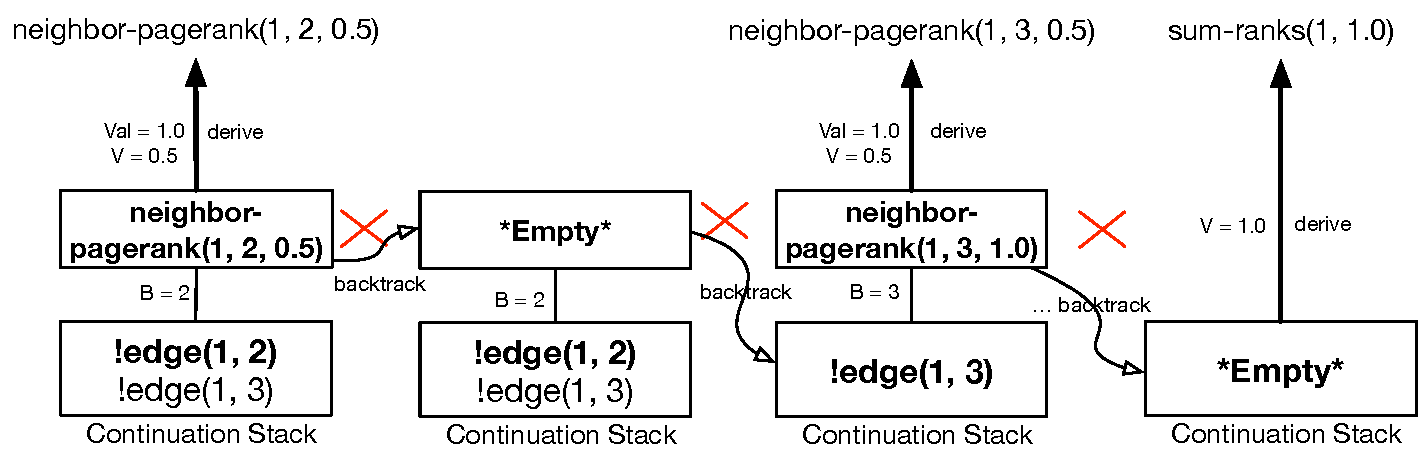
\includegraphics[width=0.85\linewidth]{figures/logical_foundations/backtrack.pdf}
   \end{center}
   \caption{Generating the PageRank aggregate.}
   \label{fig:logic:backtrack}
\end{figure}

\subsubsection{Matching}

The matching state for aggregates is 
$\matstatea{\Delta_N}{\lstack{C};
   \lstack{P}}{\Gamma}{\Delta}{\Omega}{\Delta' \rightarrow \Omega'}{\Sigma}$

\begin{enumerate}
   \item[$\Omega_N$] ordered list of remaining terms of the head of the rule to
   be derived;

   \item[$\Delta_N$] multi-set of linear facts that were still available after
   matching the body of the rule and all the previous aggregates. Note that
   $\Delta, \Xi = \Delta_N$;

   \item[$\Xi$] multi-set of linear facts used during the matching process of
   the body of the rule and all the previous aggregates;

   \item[$\Gamma_{1}$] set of persistent facts derived up to this point in the
   head of the rule;

   \item[$\Delta_{1}$] multi-set of linear facts derived up to this point in
   the head of the rule;

   \item[$\Delta'$] multi-set of linear facts consumed up to this point;

   \item[$\Omega'$] terms matched using $\Delta'$ up to this point;

   \item[$\m{agg}$] aggregate that is being matched;

   \item[$\Sigma$] the list of aggregated values;

   \item[$\lstack{C}$] continuation stack that contains both linear and persistent
   frames. The first frame must be linear;

   \item[$\lstack{P}$] initial part of the continuation stack with only persistent
   frames;

   \item[$\Delta$] multi-set of linear facts remaining up to this point in the
   matching process;

   \item[$\Omega$] ordered list of terms that need to be matched for the
   comprehension to be applied.

\end{enumerate}

Since aggregates accumulate values (from specific variables), we retrieved the
value from the $\Psi$ context. Remember that $\Psi$ is used for the
quantification connectives in the sequent calculus and in LLD is used to store
current variable bindings.

\subsubsection{Linear fact expressions}

The following two transitions deal with the case when there is a linear
fact expression in the body of the aggregate.


\begin{multline}
\transx{
   \matstatea{\deltan}{\lstack{C};
      \lstack{P}}{\Gamma}{\Delta, p_1, \Delta''}{p, \Omega}{\Delta' \rightarrow
         \Omega'}{\Sigma}
}
{
   \matstatea{\deltan}{\lframe{\Delta,
   p_1}{\Delta''}{p}{\Omega}{\Delta'}{\Omega'}, \lstack{C}; \lstack{P}}{\Gamma}{\Delta,
      \Delta''}{\Omega}{\Delta', p \rightarrow \Omega' \otimes
      p}{\Sigma}\tag{agg match p ok}
}
\end{multline}

\[
\trans{
   \matstatea{\deltan}{\lstack{C}; \lstack{P}}{\Gamma}{\Delta}{p,
      \Omega}{\Delta' \rightarrow \Omega'}{\Sigma}
}
{
   \contstatea{\deltan}{\lstack{C} ; \lstack{P}}{\Gamma}{\Sigma}
}\tag{agg match p fail}
\]


\subsubsection{Persistent fact expressions}

The transitions for dealing with persistent facts are similar to the previous
ones.



\[
\trans{
   \matstatea{\Delta_N}{\cdot;
      \lstack{P}}{\Gamma, p_1, \Gamma''}{\Delta}{\bang p, \Omega}{\Delta' \rightarrow
         \Omega'}{\Sigma}
}
{
   \matstatea{\Delta_N}{\cdot; \pframe{\Gamma''}{\Delta}{\bang
   p}{\Omega}{\Delta'}{\Omega'}, \lstack{P}}{\Gamma, p_1, \Gamma''}{\Delta}{\Omega}
   {\Delta' \rightarrow \Omega' \otimes \bang p}{\Sigma}
}
\]

\[
\trans{
   \matstatea{\Delta_N}{\lstack{C};
      \lstack{P}}{\Gamma, p_1, \Gamma''}{\Delta}{\bang p, \Omega}{\Delta' \rightarrow
         \Omega'}{\Sigma}
}
{
   \matstatea{\Delta_N}{\pframe{\Gamma''}{\Delta}{\bang
   p}{\Omega}{\Delta'}{\Omega'}, \lstack{C} ; \lstack{P}}{\Gamma, p_1, \Gamma''}{\Delta}{\Omega}
   {\Delta' \rightarrow \Omega' \otimes \bang p}{\Sigma}
}
\]


\[
\trans{
   \matstatea{\Delta_N}{\lstack{C}; \lstack{P}}{\Gamma}{\Delta}{\bang p,
      \Omega}{\Delta' \rightarrow \Omega'}{\Sigma}
}
{
   \contstatea{\Delta_N}{\lstack{C} ; \lstack{P}}{\Gamma}{\Sigma}
}
\]



\subsubsection{Deconstruct body}


\begin{multline}
\transx{
   \matstatea{\deltan}{\lstack{C};
      \lstack{P}}{\Gamma}{\Delta}{X \otimes Y, \Omega}{\Delta' \rightarrow
         \Omega'}{\Sigma}
}
{
   \matstatea{\deltan}{\lstack{C};
      \lstack{P}}{\Gamma}{\Delta}{X, Y, \Omega}{\Delta' \rightarrow
         \Omega'}{\Sigma}
} \tag{agg match $\otimes$}
\end{multline}

\begin{multline}
\transx{
   \matstatea{\deltan}{\lstack{C};
      \lstack{P}}{\Gamma}{\Delta}{\one, \Omega}{\Delta' \rightarrow
         \Omega'}{\Sigma}
}
{
   \matstatea{\deltan}{\lstack{C};
      \lstack{P}}{\Gamma}{\Delta}{\Omega}{\Delta' \rightarrow
         \Omega'}{\Sigma}
      } \tag{agg match $\one$}
\end{multline}



\subsubsection{Successful match}

When the aggregate body finally matches, we retrieve the term for variable $x$
(the aggregate variable) and add it to the list $\Sigma$.

\[
\infer[\ma{AG} \m{end}]
{\ma{AG} \Psi; \Gamma; \Delta; \Xi_N; \Gamma_{N1}; \Delta_{N1}; \Xi; \cdot;
   \lstack{C}; \lstack{P}; \Omega_N; \Delta_N; \Sigma \rightarrow \outsem}
{\fixa{AG} \Gamma; \Xi_N; \Gamma_{N1}; \Delta_{N1}; \Xi; \lstack{C}; \lstack{P}; \Omega_N;
   \Delta_N; V :: \Sigma \rightarrow \outsem & x : V : \tau \in \Psi}
\]


\subsubsection{Continuation stack update}

As we said before, to update the continuation stacks, we need remove to all the
frames except the first linear frame and remove the consumed linear facts from
the remaining frames so that they are still valid for the next application of
the aggregate.  The judgment that updates the stack has the form
$\fixstatea{\Delta}{\Xi; \Delta'}{\lstack{C};
   \lstack{P}}{\Gamma}{\Sigma}$, where:

\begin{enumerate}
   \item[$\Omega_N$] ordered list of remaining terms of the head of the rule to
   be derived;
   \item[$\Delta$] multi-set of linear facts that were still available after
   matching the body of the rule and the body of the aggregate;
   \item[$\Xi$] multi-set of linear facts used during the matching process of
   the body of the rule and all the previous aggregates;
   \item[$\Delta'$] multi-set of linear facts consumed by the aggregate body;
   \item[$\Gamma_{1}$] set of persistent facts derived by the head of the rule
   and all the previous aggregates;
   \item[$\Delta_{1}$] multi-set of linear facts derived by the head of the
   rule and all the previous aggregates;
   \item[$\m{agg}$] the current aggregate;
   \item[$\Sigma$] list of accumulated values;
   \item[$\lstack{C}, \lstack{P}$] continuation stacks for the comprehension;
   \item[$\Gamma$] set of usable persistent facts.
\end{enumerate}

\subsubsection{Remove linear continuation frames}

To remove all linear continuation frames except the first one, we simply go
through all the frames in the stack $\lstack{C}$ until only one frame remains.
This last frame and stack $\lstack{P}$ are then updated by removing $\Delta'$
from its contexts.


{\tiny
\[
\infer[\fixa ~\m{end~linear}]
{\fixa \Gamma; \Xi_N; \Gamma_{N1}; \Delta_{N1}; \Xi; (\Delta_x; \Delta''; \cdot;
      p; \Omega; \cdot; \Upsilon); P;  \aggsz{A}{B}{C}; \Omega_N; \Delta_N; T \rightarrow \Xi'; \Delta'; \Gamma'}
{\begin{split}\strans &\Xi; P; P' \\ \da \Gamma; \Xi_N, \Xi; \Gamma_{N1};
   \Delta_{N1}; B; (\Delta_x - \Xi; \Delta'' - \Xi; \cdot;& p; \Omega; \cdot;
         \Upsilon) ; P' ; \aggsz{A}{B}{C}; \Omega_N; (\Delta_N - \Xi); T &\rightarrow \Xi'; \Delta'; \Gamma'\end{split}}
\]
}

\[
\infer[\fixa \m{more}]
{\fixa \Gamma; \Xi_N; \Gamma_{N1}; \Delta_{N1}; \Xi; \_, X, C; P; AG; \Omega_N; \Delta_N; T \rightarrow \Xi'; \Delta'; \Gamma'}
{\fixa \Gamma; \Xi_N; \Gamma_{N1}; \Delta_{N1}; \Xi; X, C; P; AG; \Omega_N; \Delta_N; T \rightarrow \Xi'; \Delta'; \Gamma'}
\]

{\footnotesize
\[
\infer[\fixa \m{end~empty}]
{\fixa \Gamma; \Xi_N; \Gamma_{N1}; \Delta_{N1}; \Xi; \cdot; P; \aggsz{A}{B}{C}; \Omega_N; \Delta_N; T \rightarrow \Xi'; \Delta'; \Gamma'}
{\begin{split}\strans &\Xi; P; P' \\ \da \Gamma; \Xi_N, \Xi; \Gamma_{N1};
   \Delta_{N1}; B; \cdot ; P' ; &\aggsz{A}{B}{C}; \Omega_N; (\Delta_N - \Xi); T &\rightarrow \Xi'; \Delta'; \Gamma'\end{split}}
\]
}


\subsubsection{Aggregate backtracking}

If the aggregate match fails, we need to backtrack to the next candidate fact.
The backtracking state 
has the form
$\contstatea{\Delta_N}{\lstack{C} ; \lstack{P}}{\Gamma}{\Sigma}$, where:

\begin{enumerate}
   \item[$\Omega_N$] ordered list of remaining terms of the head of the rule to
   be derived;
   \item[$\Delta_N$] multi-set of linear facts that were still available after
   matching the body of the rule and the body of the aggregate;
   \item[$\Xi$] multi-set of linear facts used during the matching process of
   the body of the rule and all the previous aggregates;
   \item[$\Gamma_{1}$] set of persistent facts derived by the head of the rule
   and all the previous aggregates;
   \item[$\Delta_{1}$] multi-set of linear facts derived by the head of the
   rule and all the previous aggregates;
   \item[$\m{agg}$] the current aggregate;
   \item[$\Sigma$] list of accumulated values.
   \item[$\lstack{C}, \lstack{P}$] continuation stacks for the comprehension;
   \item[$\Gamma$] set of usable persistent facts.
\end{enumerate}

\paragraph{Using the $\lstack{C}$ stack}

The following 4 state transitions use the $\lstack{C}$ stack, the stack where the
first continuation frame is linear, to perform backtracking.


\begin{multline}
\transx{
   \contstatea{\deltan}{\lframe{\Delta}{p_1, \Delta''}{p}{\Omega}{\Delta'}{\Omega'}, \lstack{C} ; \lstack{P}}{\Gamma}{\Sigma}
}
{
   \matstatea{\deltan}{\lframe{\Delta,
      p_1}{\Delta''}{p}{\Omega}{\Delta'}{\Omega'}, \lstack{C}; \lstack{P}}{\Gamma}{\Delta}{p,
      \Omega}{\Delta', p_1 \rightarrow \Omega' \otimes p}{\Sigma}
} \tag{agg next p $\lstack{C}$}
\end{multline}

\begin{multline}
\transx{
   \contstatea{\deltan}{\pframe{p_1, \Gamma''}{\Delta}{\bang
   p}{\Omega}{\Delta'}{\Omega'}, \lstack{C} ; \lstack{P}}{\Gamma}{\Sigma}
}
{
   \matstatea{\deltan}{\pframe{\Gamma''}{\Delta}{\bang p}
      {\Omega}{\Delta'}{\Omega'}, \lstack{C}; \lstack{P}}{\Gamma}{\Delta}{p,
      \Omega}{\Delta' \rightarrow \Omega' \otimes \bang p}{\Sigma}
} \tag{agg next \bang p $\lstack{C}$}
\end{multline}

\[
\trans{
   \contstatea{\deltan}{\lframe{\Delta}{\cdot}{p}{\Omega}{\Delta'}{\Omega'}, \lstack{C} ; \lstack{P}}{\Gamma}{\Sigma}
}
{
   \contstatea{\deltan}{\lstack{C} ; \lstack{P}}{\Gamma}{\Sigma}
} \tag{agg  next frame $\lstack{C}$}
\]

\[
\trans{
   \contstatea{\deltan}{\pframe{\cdot}{\Delta}{\bang
   p}{\Omega}{\Delta'}{\Omega'}, \lstack{C} ; \lstack{P}}{\Gamma}{\Sigma}
}
{
   \contstatea{\deltan}{\lstack{C} ; \lstack{P}}{\Gamma}{\Sigma}
} \tag{agg next \bang frame $\lstack{C}$}
\]


\paragraph{Using the $\lstack{P}$ stack}

The following 2 state transitions rules use the $\lstack{P}$ stack instead, the stack where all
continuation frames are persistent.

\[
\infer[\conta{AG} \m{next}~\lstack{P}~\bang p]
{\conta{AG} \Gamma; \Delta_N; \Xi_N; \Gamma_{N1}; \Delta_{N1}; \cdot; f, \lstack{P}; \Omega_N; \Sigma \rightarrow \outsem}
{\begin{gathered}
   f = [p_1, \Gamma'; \Delta_N; \cdot; \bang p; \Omega; \cdot; \Upsilon] \\
   f' = [\Gamma'; \Delta_N; \cdot; \bang p; \Omega; \cdot; \Upsilon] \\
   \ma{AG} \Gamma; \Delta_N; \Xi_N; \Gamma_{N1}; \Delta_{N1}; \cdot; \Omega; \cdot;
      f', \lstack{P}; \Omega_N; \Delta_N; \Sigma \rightarrow \outsem
 \end{gathered}
}
\]

\[
\infer[\conta{AG} \m{next}~\lstack{P}~\m{empty}~\bang p]
{\conta{AG} \Gamma; \Delta_N; \Xi_N; \Gamma_{N1}; \Delta_{N1}; \cdot; f, \lstack{P}; \Omega_N; \Sigma
   \rightarrow \outsem}
{\begin{gathered}
   f =  [\cdot; \Delta_N; \cdot; \bang p; \Omega; \cdot; \Upsilon] \\
   \conta{AG} \Gamma; \Delta_N; \Xi_N; \Gamma_{N1}; \Delta_{N1}; \cdot; \lstack{P};
      \Omega_N; \Sigma \rightarrow \outsem
 \end{gathered}
}
\]


\paragraph{Aggregate done}

If both the $\lstack{C}$ and $\lstack{P}$ stacks are empty, backtracking is
impossible and the aggregate is done. The final head of the aggregate is then
derived along with the rest of the rule's head.

\[
\infer[\conta{\aggsz{A}{B}{C}} \m{end}]
{\conta{\aggsz{A}{B}{C}} \Gamma; \Delta_N; \Xi_N; \Gamma_{N1}; \Delta_{N1}; \cdot; \cdot;
   \Omega; \Sigma \rightarrow \outsem}
{\done \Gamma; \Delta_N; \Xi_N; \Gamma_{N1}; \Delta_{N1}; (\lambda x. C
      x)\Sigma,
   \Omega \rightarrow \outsem}
\]


\subsubsection{Aggregate Derivation}

After updating the continuation stacks, the subhead of the aggregate is derived.
The derivation state has the form
$\derstatea{\Delta}{\Xi}{\Gamma_1}{\Delta_1}{\Sigma}{\lstack{C};
   \lstack{P}}{\Omega}$, where:

\begin{enumerate}
   \item[$\Omega_N$] ordered list of remaining terms of the head of the rule to
   be derived;
   \item[$\Delta$] multi-set of remaining linear facts that can be used for
   the next aggregate applications.
   \item[$\Xi$] multi-set of linear facts consumed both by the body of the rule
   and previous aggregate applications;
   \item[$\Gamma_1$] set of persistent facts derived by the head of the rule,
   previous aggregates and current derivation;
   \item[$\Delta_1$] multi-set of linear facts derived by the head of the rule,
   previous aggregates and current derivation;
   \item[$\m{agg}$] current aggregate symbol;
   \item[$\Sigma$] accumulated list of values of the aggregate;
   \item[$\lstack{C}, \lstack{P}$] new continuation stacks;
   \item[$\Gamma$] set of persistent facts;
   \item[$\Omega$] ordered list of terms to derive.
\end{enumerate}

\[
\infer[\da{AG} p]
{\da{AG} \Gamma; \Delta_N; \Xi_N; \Gamma_1; \Delta_1; p, \Omega; \lstack{C}; \lstack{P}; \Omega_N;
   \Sigma \rightarrow \outsem}
{\da{AG} \Gamma; \Delta_N; \Xi_N; \Gamma_1; \Delta_1, p; \Omega; \lstack{C}; \lstack{P}; \Omega_N;
   \Sigma \rightarrow \outsem}
\]

\[
\infer[\da{AG} \bang p]
{\da{AG} \Gamma; \Delta_N; \Xi_N; \Gamma_1; \Delta_1; \bang p, \Omega; \lstack{C};
   \lstack{P}; \Omega_N; \Sigma \rightarrow \outsem}
{\da{AG} \Gamma; \Delta_N; \Xi_N; \Gamma_1, p; \Delta_1; \Omega; \lstack{C}; \lstack{P}; \Omega_N;
   \Sigma \rightarrow \outsem}
\]

\[
\infer[\da{AG} \otimes]
{\da{AG} \Gamma; \Delta_N; \Xi_N; \Gamma_1; \Delta_1; A \otimes B, \Omega; \lstack{C}; \lstack{P}; \Omega_N;
   \Sigma \rightarrow \outsem}
{\da{AG} \Gamma; \Delta_N; \Xi_N; \Gamma_1; \Delta_1; A, B, \Omega; \lstack{C}; \lstack{P}; \Omega_N;
   \Sigma \rightarrow \outsem}
\]

\[
\infer[\da{AG} \m{end}]
{\da{AG} \Gamma; \Delta_N; \Xi_N; \Gamma_1; \Delta_1; \cdot; \lstack{C}; \lstack{P}; \Omega_N;
   \Sigma \rightarrow \outsem}
{\conta{AG} \Gamma; \Delta_N; \Xi_N; \Gamma_1; \Delta_1; \lstack{C}; \lstack{P}; \Omega_N; \Sigma
   \rightarrow \outsem}
\]



This completes the specification of LLD.




\section{Soundness Proof}

Now that we have presented both the HLD and LLD semantics, we are in position to
start building our soundness theorem.  The soundness theorem proves that if a
rule was successfully derived in the LLD semantics then it can also be derived
in the HLD semantics. Since the HLD semantics are so close to linear logic, we
prove that our language has a determined, correct, proof search behavior when
executing programs. However, the completeness theorem cannot be proven since LLD
lacks the non-determinism inherent in HLD.

First and foremost, we need to prove some auxiliary theorems and definitions
that will be used during the soundness theorem.

\subsection{Soundness Of Matching}

The soundness theorem will be proven into two main steps. First, we prove that
performing a rule match at LLD is sound in relation to HLD and then we prove
that the derivation of the rule's RHS is also sound.

In order to prove the soundness of matching, we want to reconstitute a valid
match $\mz{\Gamma}{\Delta}{A}$ in HLD from machine steps in LLD. Our machine
specification already includes a built-in $\mz{\Gamma}{\Delta}{A}$ judgment that
can be used to prove soundness immediately. However, we need to prove that
every state transition preserves the well-formedness of the machine from the
previous definitions.

\begin{theorem}[Rule transitions preserve well-formedness]
Given a rule $A \lolli B$, consider a triplet $T = A; \Gamma; \Delta_{N}$.
If a state $s_1$ is well-formed in relation to $T$ and $\trans{s_1}{s_2}$ then
$s_2$ is also well-formed.
\end{theorem}
\begin{proof}
Case by case analysis.
\begin{itemize}
\item match p ok: simple manipulation of multi-set equality and use of
equivalence rules.
\item match p fail: trivial.
\item match \bang p ok: multi-set manipulation and use of
equivalence rules.
\item match \bang p fail: trivial.
\item match $\one$: use of term equivalence rules.
\item match $\bang$: use of term equivalence rules.
\item next p: simple multi-set manipulation.
\item next frame: trivial.
\item next \bang frame: trivial.
\end{itemize}
\end{proof}

Given this result, we now need to prove that from an initial matching state, we
end up with a final matching state. The final matching state will include the
soundness result since all state transitions preserve well-formedness.
However, LLD may fail during matching, therefore the match lemma needs to handle
unsuccessful matches. In order to be able to use induction, we must assume a
general matching state that  already contains some continuation frames in
stack $\lstack{C}$. The lemma also needs to relate the matching state with the
backtracking state since there is a need to backtrack during the matching
process. Apart from an unsuccessful match, we deal with two situations
during a successful match: (1) we succeed without needing to backtrack to a
frame in stack $\lstack{C}$ or (2) we need to backtrack to a frame in
$\lstack{C}$. The complete lemma is stated and proven below.


\begin{lemma}[LHS match result]\label{thm:body_match}
   
Given a rule $A \lolli H$, consider a triplet $T = A; \Gamma; \Delta_{N}$ and a
context $\Delta_{N} = \Delta_1, \Delta_2, \Xi$.

If $s_1 = \matstateb{A \lolli B}{\rulestk}{\lstack{C}}{\Gamma}{\Delta_1,
   \Delta_2}{\Omega}{\Delta' \rightarrow \Omega'\Psi}{\Psi}$
is well-formed in relation to $T$ and $\transs{s_1}{s_2}$ then:

\begin{itemize}[leftmargin=*]
   \item Match succeeds with no backtracking to frames of stack $\lstack{C}$:
   \begin{itemize}[leftmargin=\secondm]
      \item $s_2 = \matstateb{A \lolli B}{\rulestk}{\lstack{C''},
         \lstack{C}}{\Gamma}{\Delta_1}{\cdot}{\Delta', \Delta_2 \rightarrow
         \Omega'\Psi \otimes split(\Omega)\Psi_2}{\m{extend}(\Psi, \Psi2)}$
      %\item $\mo \Gamma; \Delta_1; \Xi, \Delta_2; \cdot; H; \lstack{C''}, \lstack{C}; \lstack{R} \rightarrow \outsem$ (well-formed in relation to $T$)
      %\item $\mo \Gamma; \Delta_1; \Xi, \Delta_2; \Omega; H; \lstack{C}; (\cdot, \deltan) \rightarrow \outsem$ (well-formed in relation to $T$)
   \end{itemize}

   
   \item Match fails:
   \begin{itemize}[leftmargin=\secondm]
      \item $s_2 = \contstate{A \lolli B}{\rulestk}{\cdot}{\Gamma}$
   \end{itemize}

   \item Match succeeds with backtracking to a linear frame:
   \begin{itemize}[leftmargin=\secondm]
      \item $s_2 = \matstate{A \lolli B}{\rulestk}{\lstack{C'''}, f',
         \lstack{C''}}{\Gamma}{\Delta_c}{\cdot}{\Delta'_f, p_2, \Delta''_f \rightarrow
         \Omega_f \otimes p \otimes split(\Omega'_f)}$

      \item $\lstack{C} = \lstack{C'}, f, \lstack{C''}$

      \item $f = \lframe{\Delta_a}{\Delta_{b_1}, p_2, \Delta_{b_2}}{p}{\Omega_f}{\Delta_f'}{\Omega_f'}$
      turns into $f' = \lframe{\Delta_a, \Delta_{b_1}, p_2}
{\Delta_{b_2}}{p}{\Omega_f}{\Delta_f'}{\Omega_f'}$

      \item $\Delta_c = (\Delta_1, \Delta_2, \Delta') - (\Delta'_f, \Delta''_f, p_2)$
   \end{itemize}

   \item Match succeeds with backtracking to a persistent frame:
   \begin{itemize}[leftmargin=\secondm]
      \item $s_2 = \matstate{A \lolli B}{\rulestk}{\lstack{C'''}, f',
         \lstack{C''}}{\Gamma}{\Delta_{c_1}}{\cdot}{\Delta'_f, \Delta_{c_2}
            \rightarrow \Omega_f \otimes \bang p \otimes split(\Omega'_f)}$
      \item $\lstack{C} = \lstack{C'}, f, \lstack{C''}$

      \item $f = \pframe{\Gamma_1, p_2,
         \Gamma_2}{\Delta_{c_1}, \Delta_{c_2}}{\bang p}{\Omega_f}{\Delta'_f}{\Omega'_f}$
      turns into $f' = \pframe{\Gamma_2}{\Delta_{c_1},
         \Delta_{c_2}}{\bang p}{\Omega_f}{\Delta'_f}{\Omega'_f}$

      \item $\Delta_{c_1}, \Delta_{c_2} = (\Delta_1, \Delta_2,
            \Delta') - \Delta'_f$
   \end{itemize}


\end{itemize}

If $s_1 = \contstate{A \lolli B}{\rulestk}{\lstack{C}}{\Gamma}$ 
is well-formed in relation to $T$ and $\transs{s_1}{s_2}$ then either:

\begin{itemize}[leftmargin=*]
   
   \item Match fails:
   \begin{itemize}[leftmargin=\secondm]
      \item $s_2 = \contstate{A \lolli B}{\rulestk}{\cdot}{\Gamma}$
   \end{itemize}

   \item Match succeeds with backtracking to a linear frame:
   \begin{itemize}[leftmargin=\secondm]
      \item $s_2 = \matstate{A \lolli B}{\rulestk}{\lstack{C'''}, f',
         \lstack{C''}}{\Gamma}{\Delta_c}{\cdot}{\Delta'_f, p_2, \Delta''_f \rightarrow
         \Omega_f \otimes p \otimes split(\Omega'_f)}$

      \item $\lstack{C} = \lstack{C'}, f, \lstack{C''}$

      \item $f = \lframe{\Delta_a}{\Delta_{b_1}, p_2, \Delta_{b_2}}{p}{\Omega_f}{\Delta_f'}{\Omega_f'}$
      turns into $f' = \lframe{\Delta_a, \Delta_{b_1}, p_2}
{\Delta_{b_2}}{p}{\Omega_f}{\Delta_f'}{\Omega_f'}$

      \item $\Delta_c = (\Delta_1, \Delta_2, \Delta') - (\Delta'_f, \Delta''_f, p_2)$
   \end{itemize}

   \item Match succeeds with backtracking to a persistent frame:
   \begin{itemize}[leftmargin=\secondm]
      \item $s_2 = \matstate{A \lolli B}{\rulestk}{\lstack{C'''}, f',
         \lstack{C''}}{\Gamma}{\Delta_{c_1}}{\cdot}{\Delta'_f, \Delta_{c_2}
            \rightarrow \Omega_f \otimes \bang p \otimes split(\Omega'_f)}$
      \item $\lstack{C} = \lstack{C'}, f, \lstack{C''}$

      \item $f = \pframe{\Gamma_1, p_2,
         \Gamma_2}{\Delta_{c_1}, \Delta_{c_2}}{\bang p}{\Omega_f}{\Delta'_f}{\Omega'_f}$
      turns into $f' = \pframe{\Gamma_2}{\Delta_{c_1},
         \Delta_{c_2}}{\bang p}{\Omega_f}{\Delta'_f}{\Omega'_f}$

      \item $\Delta_{c_1}, \Delta_{c_2} = (\Delta_1, \Delta_2,
            \Delta') - \Delta'_f$
   \end{itemize}

\end{itemize}
\end{lemma}

\begin{proof}
   Proof by lexicographic induction on the state transitions. First on the size of
   $\Omega$ and then on the size of the second argument of the linear frame or
   on the first argument of the linear frame and then on the size of the stack
   $\lstack{C}$.
   Sub-cases:

\begin{itemize}[leftmargin=*]
\item match p ok

Induction on the state with a new frame ($\Omega$ is smaller). Trivial if match
fails, otherwise it succeeds by adding new frames (including the new frame) or by backtracking.

\item match p fail

State gets smaller (see next).

\item match \bang p ok

Use the strategy used for match p ok.

\item match \bang p fail: state gets smaller.

\item match $\one$: trivial because $split$ removes $\one$.

\item match $\bang$: same.
\item next p

Frame gets smaller so we can use the induction hypothesis:
\begin{itemize}
   \item Match fails: trivial.
   \item Match succeeds with no backtracking: the frame that was updated is the
   successful frame to backtrack to.
   \item Match succeeds with backtracking: the frame $f \in \lstack{C}$ is the
   frame we need.
\end{itemize}

\item next frame: stack gets smaller.
\item next \bang frame: stack gets smaller (see above).
\end{itemize}

\end{proof}


For the induction hypothesis to be applicable in Lemma~\ref{thm:body_match}
there must be a relation between the machine states.  We can define a
lexicographic ordering $s_1 \prec s_2$, meaning that $s_1$ has a smaller number
of remaining steps than state $s_2$.  The specific ordering is as follows:

\begin{enumerate}[leftmargin=*]
   \item $\contstate{A \lolli B}{\rulestk}{\lstack{C}}{\Gamma} \prec
   \contstate{A \lolli B}{\rulestk}{\lstack{C'}, \lstack{C}}{\Gamma}$

   The continuation must use the top of the stack $\lstack{C'}$ before using
   $\lstack{C}$;

   \item $\contstate{A \lolli B}{\rulestk}{\lframe{\Delta,
      \Delta_1}{\Delta_2}{p}{\Omega}{\Delta_f}{\Omega_f}, \lstack{C}}{\Gamma}
      \prec \contstate{A \lolli B}{\rulestk}{\lframe{\Delta}{\Delta_1,
         \Delta_2}{p}{\Omega}{\Delta_f}{\Omega_f}, \lstack{C}}{\Gamma}$

   A continuation frame with more candidates has more steps to do than a frame with less candidates;

   \item $\contstate{A \lolli B}{\rulestk}{\pframe{\Gamma_1}{\Delta}{\bang
      p}{\Omega}{\Delta_f}{\Omega_f}}{\Gamma} \prec \contstate{A \lolli
         B}{\rulestk}{\pframe{\Gamma_1, \Gamma_2}{\Delta}{\bang
            p}{\Omega}{\Delta_f}{\Omega_f}}{\Gamma}$

      Same as the previous one;

   \item $\contstate{A \lolli B}{\rulestk}{\lstack{C}}{\Gamma} \prec
      \matstate{A \lolli B}{\rulestk}{\lstack{C'},
         \lstack{C}}{\Gamma}{\Delta}{\Omega}{\Delta' \rightarrow \Omega'}$

   \item $\matstate{A \lolli
      B}{\rulestk}{\lstack{C}}{\Gamma}{\Delta}{\Omega}{\Delta' \rightarrow
         \Omega'} \prec \contstate{A \lolli B}{\rulestk}{\lstack{C'},
            \lstack{C}}{\Gamma}$
   \item $\matstate{A \lolli B}{\rulestk}{\lstack{C'},
      \lstack{C}}{\Gamma}{\Delta_1}{\Omega_1}{\Delta'_1 \rightarrow \Omega'_1} \prec
      \matstate{A \lolli
         B}{\rulestk}{\lstack{C}}{\Gamma}{\Delta_2}{\Omega_2}{\Delta'_2 \rightarrow
            \Omega'_2}$

   Adding continuation frames to the stack makes the proof smaller as long as
   $\Omega$ is also smaller; 

   \item $\matstate{A \lolli B}{\rulestk}{\lstack{C'}, \lframe{\Delta_f,
      \Delta_{f_1}}{\Delta_{f_2}}{p}{\Omega_f}{\Delta'_f}{\Omega'_f},
   \lstack{C}}{\Gamma}{\Delta_1}{\Omega_1}{\Delta'_1 \rightarrow \Omega'_1}$\\
   \hspace*{1cm} $\prec \matstate{A \lolli B}{\rulestk}{\lstack{C''},
      \lframe{\Delta_f}{\Delta_{f_1},
         \Delta_{f_2}}{p}{\Omega_f}{\Delta'_f}{\Omega'_f},
      \lstack{C}}{\Gamma}{\Delta_2}{\Omega_2}{\Delta'_2 \rightarrow \Omega'_2}$

   \item $\matstate{A \lolli B}{\rulestk}{\lstack{C'},
      \pframe{\Gamma_1}{\Delta_f}{\bang p}{\Omega_f}{\Delta_f}{\Omega_f},
   \lstack{C}}{\Gamma}{\Delta_1}{\Omega_1}{\Delta'_1 \rightarrow \Omega'_1}$\\
   \hspace*{1cm} $\prec \matstate{A \lolli B}{\rulestk}{\lstack{C''},
      \pframe{\Gamma_1, \Gamma_2}{\Delta_f}{\bang p}{\Omega_f}{\Delta'_f}{\Omega'_f},
      \lstack{C}}{\Gamma}{\Delta_2}{\Omega_2}{\Delta'_2 \rightarrow \Omega'_2}$

\end{enumerate}

\subsection{Soundness Of Derivation}

Proving that the derivation of the rule's RHS is sound is trivial except
for comprehensions and aggregates. LLD deterministically computes the number of
available aggregates to apply while HLD "guesses" the number of required
derivations.  In the next two sections, we show how to prove the soundness of
aggregates. The strategy for proving for proving both is identical due to their
inherent similarities.

\subsection{Aggregate Soundness}


Proving that deriving an aggregate in LLD is sound in relation to HLD is built
from 4 results: (1) proving that matching the aggregate's LHS is sound in
relation to HLD; (2) proving that updating the continuation stacks makes them
suitable for use in the next aggregate applications; (3) proving that deriving
the aggregate's RHS is sound in relation to HLD; (4) proving that we can
apply as many aggregates as the database allows.

\begin{lemma}[Aggregate LHS match]\label{thm:aggregate_body_match}
Consider an aggregate $\m{agg}$, where $\Pi(\m{agg}) = \forall_{\widehat{v}, \Sigma'}.
   (\defstwo{agg}{\widehat{v}}{\Sigma'} \lolli ((\lambda x. C x)\Sigma' \with (\forall_{\widehat{x}, \sigma}.
                                                (A \lolli B \otimes
                                                 \defstwo{agg}{\widehat{v}}{\sigma
                                                 ::\Sigma'}))))$,
a triplet $T = A; \Gamma; \Delta_{N}$ and a context $\Delta_{N} = \Delta_1,
  \Delta_2, \Delta'$.

  If $s_1 = \matstatea{\Delta_N}{\lstack{C};
      \lstack{P}}{\Gamma}{\Delta_1, \Delta_2}{\Omega}{\Delta' \rightarrow
         \Omega'}{\Sigma}$ is well-formed in relation to $T$ and
         $\transs{s_1}{s_2}$ then either:

\begin{itemize}[leftmargin=*]
   \item Match succeeds with no backtracking to frames of stack $\lstack{C}$
   or $\lstack{P}$ ($\lstack{C} \neq \cdot$):

   \begin{itemize}[leftmargin=\secondm]
      \item $s_2 = \matstatea{\Delta_N}{\lstack{C'}, \lstack{C}; \lstack{P'},
         \lstack{P}}{\Gamma}{\Delta_1}{\cdot}{\Delta', \Delta_2 \rightarrow \Omega' \otimes split(\Omega)}{\Sigma}$
   \end{itemize}

   \item Match succeeds with no backtracking to frames of stack $\lstack{P}$
($\lstack{C} = \cdot$):
\begin{itemize}[leftmargin=\secondm]
   \item $\mz \Gamma; \Delta_2 \rightarrow A$
   \item $\ma{AG} \Gamma; \Delta_1; \Xi_N; \Gamma_{N1}; \Delta_{N1}; \Xi,
      \Delta_2; \cdot; \lstack{C'}; \lstack{P'}, \lstack{P}; \Omega_N; \Delta_N;
      \Sigma \rightarrow \outsem$ (well-formed in relation to $T$)
\end{itemize}

\item Match succeeds with backtracking to a linear continuation frame in
stack $\lstack{C}$ ($\lstack{C} \neq \cdot$):

\begin{itemize}[leftmargin=\secondm]
   \item $\mz \Gamma; \Xi_1, \dotsc, \Xi_m, p_2, \Xi_c$
   \item $\exists_{f \in \lstack{C}}. f = (\Delta_a; \Delta_{b_1}, p_2,
         \Delta_{b_2}; p; \Xi_1, \dotsc, \Xi_m; \Omega_1, \dotsc,
         \Omega_k; \Lambda_1, \dotsc, \Lambda_m; \Upsilon_1, \dotsc,
         \Upsilon_n)$
   \item $\lstack{C} = \lstack{C'}, f, \lstack{C''}$
   \item $f$ turns into $f' = (\Delta_a, \Delta_{b_1}, p_2;
         \Delta_{b_2}; p; \Xi_1, \dotsc, \Xi_m;
         \Omega_1, \dotsc, \Omega_k; \Lambda_1, \dotsc, \Lambda_m;
         \Upsilon_1, \dotsc, \Upsilon_n)$
   \item $\ma{AG} \Gamma; \Delta_c; \Xi_N; \Gamma_{N1}; \Delta_{N1}; \Xi_1,
      \dotsc, \Xi_m, p_2, \Xi_c; \cdot; \lstack{C'''}, f', \lstack{C''}; \lstack{P};
      \Omega_N; \Delta_N; \Sigma \rightarrow \outsem$ (well-formed in relation to $T$)
   \item $\Delta_c = (\Delta_1, \Delta_2, \Xi) - (\Xi_1, \dotsc, \Xi_m,
         p_2, \Xi_c)$
\end{itemize}

\item Match succeeds with backtracking to a persistent continuation frame
in stack $\lstack{C}$ ($\lstack{C} \neq \cdot$):
\begin{itemize}[leftmargin=\secondm]
   \item $\mz \Gamma; \Delta_{c_2}, \Xi_1, \dotsc, \Xi_m \rightarrow A$
   \item $\exists_{f \in \lstack{C}}. f = [\Gamma_1, p_2, \Gamma_2; \Delta_{c_1},
      \Delta_{c_2}; \Xi_1, \dotsc, \Xi_m; \bang p; \Omega_1, \dotsc, \Omega_k;
      \Lambda_1, \dotsc, \Lambda_m; \Upsilon_1, \dotsc, \Upsilon_n]$
   \item $\lstack{C} = \lstack{C'}, f, \lstack{C''}$
   \item $f$ turns into $f' = [\Gamma_2; \Delta_{c_1}, \Delta_{c_2};
      \Xi_1, \dotsc, \Xi_m; \bang p; \Omega_1, \dotsc, \Omega_k; \Lambda_1,
      \dotsc, \Lambda_m; \Upsilon_1, \dotsc, \Upsilon_n]$
   \item $\ma{AG} \Gamma; \Delta_{c_1}; \Xi_N; \Gamma_{N1}; \Delta_{N1};
      \Delta_{c_2}, \Xi_1, \dotsc, \Xi_m; \cdot; \lstack{C'''}, f', \lstack{C''}; \lstack{P};
      \Omega_N; \Delta_N; \Sigma \rightarrow \outsem$ (well-formed in relation to $T$)
   \item $\Delta_{c_1}, \Delta_{c_2} = (\Delta_1, \Delta_2, \Xi) - (\Xi_1, \dotsc, \Xi_m)$
\end{itemize}

\item Match succeeds with backtracking to a persistent continuation frame
in stack $\lstack{P}$ ($\lstack{C} = \cdot$):
   \begin{itemize}[leftmargin=\secondm]
      \item $\mz \Gamma; \Delta_{c_2}, \Xi_1, \dotsc, \Xi_m \rightarrow A$
      \item $\exists_{f \in \lstack{P}}. f = [\Gamma_1, p_2, \Gamma_2; \Delta_{c_1}, \Delta_{c_2};
   \Xi_1, \dotsc, \Xi_m; \bang p; \Omega_1, \dotsc, \Omega_k; \Lambda_1,
   \dotsc, \Lambda_m; \Upsilon_1, \dotsc, \Upsilon_n]$
      \item $\lstack{P} = \lstack{P'}, f, \lstack{P''}$
      \item $f$ turns into $f' = [\Gamma_2; \Delta_{c_1},
         \Delta_{c_2}; \Xi_1, \dotsc, \Xi_m; \bang p; \Omega_1, \dotsc,
         \Omega_k; \Lambda_1, \dotsc, \Lambda_m; \Upsilon_1, \dotsc, \Upsilon_n]$
      \item $\ma{AG} \Gamma; \Delta_{c_1}; \Xi_N; \Gamma_{N1}; \Delta_{N1};
         \Delta_{c_2}, \Xi_1, \dotsc, \Xi_m; \cdot; \lstack{C'}; \lstack{P'''}, f', \lstack{P''};
         \Omega_N; \Delta_N; \Sigma \rightarrow \outsem$
         (well-formed in relation to $T$)
      \item $\Delta_{c_1}, \Delta_{c_2} = (\Delta_1, \Delta_2, \Xi) - (\Xi_1, \dotsc,
            \Xi_m)$
   \end{itemize}


\end{itemize}

If $\contstatea{\Delta_N}{\lstack{C}; \lstack{P}}{\Gamma}{\Sigma}$ is
well-formed in relation to $T$ then either:

\begin{itemize}[leftmargin=*]
   \item Match succeeds with no backtracking to frames of stack $\lstack{P}$
($\lstack{C} = \cdot$):
\begin{itemize}[leftmargin=\secondm]
   \item $\mz \Gamma; \Delta_2 \rightarrow A$
   \item $\ma{AG} \Gamma; \Delta_1; \Xi_N; \Gamma_{N1}; \Delta_{N1}; \Xi,
      \Delta_2; \cdot; \lstack{C'}; \lstack{P'}, \lstack{P}; \Omega_N; \Delta_N;
      \Sigma \rightarrow \outsem$ (well-formed in relation to $T$)
\end{itemize}

\item Match succeeds with backtracking to a linear continuation frame in
stack $\lstack{C}$ ($\lstack{C} \neq \cdot$):

\begin{itemize}[leftmargin=\secondm]
   \item $\mz \Gamma; \Xi_1, \dotsc, \Xi_m, p_2, \Xi_c$
   \item $\exists_{f \in \lstack{C}}. f = (\Delta_a; \Delta_{b_1}, p_2,
         \Delta_{b_2}; p; \Xi_1, \dotsc, \Xi_m; \Omega_1, \dotsc,
         \Omega_k; \Lambda_1, \dotsc, \Lambda_m; \Upsilon_1, \dotsc,
         \Upsilon_n)$
   \item $\lstack{C} = \lstack{C'}, f, \lstack{C''}$
   \item $f$ turns into $f' = (\Delta_a, \Delta_{b_1}, p_2;
         \Delta_{b_2}; p; \Xi_1, \dotsc, \Xi_m;
         \Omega_1, \dotsc, \Omega_k; \Lambda_1, \dotsc, \Lambda_m;
         \Upsilon_1, \dotsc, \Upsilon_n)$
   \item $\ma{AG} \Gamma; \Delta_c; \Xi_N; \Gamma_{N1}; \Delta_{N1}; \Xi_1,
      \dotsc, \Xi_m, p_2, \Xi_c; \cdot; \lstack{C'''}, f', \lstack{C''}; \lstack{P};
      \Omega_N; \Delta_N; \Sigma \rightarrow \outsem$ (well-formed in relation to $T$)
   \item $\Delta_c = (\Delta_1, \Delta_2, \Xi) - (\Xi_1, \dotsc, \Xi_m,
         p_2, \Xi_c)$
\end{itemize}

\item Match succeeds with backtracking to a persistent continuation frame
in stack $\lstack{C}$ ($\lstack{C} \neq \cdot$):
\begin{itemize}[leftmargin=\secondm]
   \item $\mz \Gamma; \Delta_{c_2}, \Xi_1, \dotsc, \Xi_m \rightarrow A$
   \item $\exists_{f \in \lstack{C}}. f = [\Gamma_1, p_2, \Gamma_2; \Delta_{c_1},
      \Delta_{c_2}; \Xi_1, \dotsc, \Xi_m; \bang p; \Omega_1, \dotsc, \Omega_k;
      \Lambda_1, \dotsc, \Lambda_m; \Upsilon_1, \dotsc, \Upsilon_n]$
   \item $\lstack{C} = \lstack{C'}, f, \lstack{C''}$
   \item $f$ turns into $f' = [\Gamma_2; \Delta_{c_1}, \Delta_{c_2};
      \Xi_1, \dotsc, \Xi_m; \bang p; \Omega_1, \dotsc, \Omega_k; \Lambda_1,
      \dotsc, \Lambda_m; \Upsilon_1, \dotsc, \Upsilon_n]$
   \item $\ma{AG} \Gamma; \Delta_{c_1}; \Xi_N; \Gamma_{N1}; \Delta_{N1};
      \Delta_{c_2}, \Xi_1, \dotsc, \Xi_m; \cdot; \lstack{C'''}, f', \lstack{C''}; \lstack{P};
      \Omega_N; \Delta_N; \Sigma \rightarrow \outsem$ (well-formed in relation to $T$)
   \item $\Delta_{c_1}, \Delta_{c_2} = (\Delta_1, \Delta_2, \Xi) - (\Xi_1, \dotsc, \Xi_m)$
\end{itemize}

\item Match succeeds with backtracking to a persistent continuation frame
in stack $\lstack{P}$ ($\lstack{C} = \cdot$):
   \begin{itemize}[leftmargin=\secondm]
      \item $\mz \Gamma; \Delta_{c_2}, \Xi_1, \dotsc, \Xi_m \rightarrow A$
      \item $\exists_{f \in \lstack{P}}. f = [\Gamma_1, p_2, \Gamma_2; \Delta_{c_1}, \Delta_{c_2};
   \Xi_1, \dotsc, \Xi_m; \bang p; \Omega_1, \dotsc, \Omega_k; \Lambda_1,
   \dotsc, \Lambda_m; \Upsilon_1, \dotsc, \Upsilon_n]$
      \item $\lstack{P} = \lstack{P'}, f, \lstack{P''}$
      \item $f$ turns into $f' = [\Gamma_2; \Delta_{c_1},
         \Delta_{c_2}; \Xi_1, \dotsc, \Xi_m; \bang p; \Omega_1, \dotsc,
         \Omega_k; \Lambda_1, \dotsc, \Lambda_m; \Upsilon_1, \dotsc, \Upsilon_n]$
      \item $\ma{AG} \Gamma; \Delta_{c_1}; \Xi_N; \Gamma_{N1}; \Delta_{N1};
         \Delta_{c_2}, \Xi_1, \dotsc, \Xi_m; \cdot; \lstack{C'}; \lstack{P'''}, f', \lstack{P''};
         \Omega_N; \Delta_N; \Sigma \rightarrow \outsem$
         (well-formed in relation to $T$)
      \item $\Delta_{c_1}, \Delta_{c_2} = (\Delta_1, \Delta_2, \Xi) - (\Xi_1, \dotsc,
            \Xi_m)$
   \end{itemize}

\end{itemize}
\end{lemma}

Proving this particular lemma follows the same strategy used for
Lemma~\ref{thm:body_match}. Next, we need to prove that, when matching succeeds,
the continuation stack is corrected for the next application of the aggregate.
Note that the aggregate value is appended to $\Sigma$ after the stack is
corrected.

\begin{theorem}[From update to derivation]\label{thm:agg_from_update_to_derivation}
Consider an aggregate $\m{agg}$, where $\Pi(\m{agg}) = \forall_{\widehat{v}, \Sigma'}.
   (\defstwo{agg}{\widehat{v}}{\Sigma'} \lolli ((\lambda x. C x)\Sigma' \with (\forall_{\widehat{x}, \sigma}.
                                                (A \lolli B \otimes
                                                 \defstwo{agg}{\widehat{v}}{\sigma
                                                 ::\Sigma'}))))$,
a triplet $T = A; \Gamma; \Delta_{N}$ and that $\Delta_{N} = \Delta,
  \Delta'$.
A well-formed stack update
$\fixstatea{\Delta}{\Xi; \Delta'}{\lstack{C}; \lstack{P}}{\Gamma}{\Sigma}$
implies
$\derstatea{\Delta}{\Xi, \Delta'}{\Gamma_{N1}}{\Delta_{N1}}{V :: \Sigma}{f';
   \lstack{P'}}{B\{\Psi(\widehat{x}), V / \widehat{x}, \sigma\}}$,
where:

\begin{itemize}[leftmargin=*]
   \item If $\lstack{C} = \cdot$ then $\lstack{C'} = \cdot$

   \item If $\lstack{C} = \lstack{C''},
   \lframe{\Delta_a}{\Delta_b}{p}{\Omega}{\cdot}{\Omega'}$
   then $\lstack{C'} = \lframe{\Delta_a - \Delta'}{\Delta_b -
      \Delta'}{p}{\Omega}{\cdot}{\Omega'}$

   \item $\lstack{P'}$ is the transformation of stack $\lstack{P}$, where for every frame $f \in
   \lstack{P}$ of the form $\pframe{\Gamma'}{\Delta_N}{\bang
      p}{\Omega}{\cdot}{\Omega'}$
   will turn into $f' = \pframe{\Gamma'}{\Delta_N-\Delta'}{\bang
      p}{\Omega}{\cdot}{\Omega'}$

\end{itemize}
\end{theorem}
\begin{proof}
Use induction on the size of the stack $\lstack{C}$.
\end{proof}


\begin{corollary}[Match to derivation]\label{thm:agg_match_to_derivation}
Consider an aggregate $\m{agg}$, where $\Pi(\m{agg}) = \forall_{\widehat{v}, \Sigma'}.
   (\defstwo{agg}{\widehat{v}}{\Sigma'} \lolli ((\lambda x. C x)\Sigma' \with (\forall_{\widehat{x}, \sigma}.
                                                (A \lolli B \otimes
                                                 \defstwo{agg}{\widehat{v}}{\sigma
                                                 ::\Sigma'}))))$,
a triplet $T = A; \Gamma; \Delta_{N}$ and that $\Delta_{N} = \Delta,
  \Delta'$.

A well-formed $\matstatea{\Delta_N}{\lstack{C}; \lstack{P}}{\Gamma}{\Delta}{\cdot}{\Delta' \rightarrow \Omega'}{\Sigma}$
implies
$\derstatea{\Delta}{\Xi, \Delta'}{\Gamma_{N1}}{\Delta_{N1}}{V :: \Sigma}{f';
   \lstack{P'}}{B\{\Psi(\widehat{x}), V / \widehat{x}, \sigma\}}$,
where:
   
\begin{itemize}[leftmargin=*]
   \item If $\lstack{C} = \cdot$ then $\lstack{C'} = \cdot$

   \item If $\lstack{C} = \lstack{C''},
   \lframe{\Delta_a}{\Delta_b}{p}{\Omega}{\cdot}{\Omega'}$
   then $\lstack{C'} = \lframe{\Delta_a - \Delta'}{\Delta_b -
      \Delta'}{p}{\Omega}{\cdot}{\Omega'}$

   \item $\lstack{P'}$ is the transformation of stack $\lstack{P}$, where for every frame $f \in
   \lstack{P}$ of the form $\pframe{\Gamma'}{\Delta_N}{\bang
      p}{\Omega}{\cdot}{\Omega'}$
   will turn into $f' = \pframe{\Gamma'}{\Delta_N-\Delta'}{\bang
      p}{\Omega}{\cdot}{\Omega'}$

\end{itemize}
\end{corollary}

\begin{proof}
Invert the assumption and then apply Theorem~\ref{thm:agg_from_update_to_derivation}.
\end{proof}


\paragraph{Aggregate Derivation}

We have just seen that after a single aggregate application, we add a value $V$
to the $\Sigma$ context and that the continuation stacks are now valid.
Now, we need to prove that deriving the aggregate's RHS
is sound in relation to HLD by using the new stacks.

\begin{theorem}[Aggregate derivation soundness]\label{thm:aggregate_derivation}
If $\derstatea{\Delta_N}{\Xi_N}{\Gamma_{N1}}{\Delta_{N1}}{\Sigma}{\lstack{C}; \lstack{P}}{\Omega_1,
\dotsc, \Omega_n}$ then:

\begin{itemize}[leftmargin=*]
   \item $\derstatea{\Delta_N}{\Xi_N}{\Gamma_{N1}, \Gamma_1, \dotsc,
      \Gamma_n}{\Delta_{N1}, \Delta_1, \dotsc, \Delta_n}{\Sigma}{\lstack{C};
         \lstack{P}}{\cdot}$

   \item If $\dz{\Gamma}{\Pi}{\Delta_N}{\Xi_N}{\Gamma_{N1}, \Gamma_1, \dotsc,
         \Gamma_n}{\Delta_{N1}, \Delta_1, \dotsc, \Delta_n}{\Omega_x}{\outsem}$ then\\
         \hspace{2cm}
   $\dz{\Gamma}{\Pi}{\Delta_N}{\Xi_N}{\Gamma_{N1}}{\Delta_{N1}}{\Omega_1, \dotsc,
   \Omega_n, \Omega_x}{\outsem}$

\end{itemize}
\end{theorem}

\begin{proof}
Straightforward induction on $\Omega_1, \dotsc, \Omega_n$.
\end{proof}


\paragraph{Multiple Aggregate Derivation} We now prove that it is possible
to apply an aggregate several times in order to a get multiple values (one per
application). In turn, we also conclude important results for the
soundness of the aggregate computation mechanism.

\begin{theorem}[Multiple aggregate derivation]\label{thm:multiple_aggregate_derivation}
Consider an aggregate $\m{agg}$, where $\Pi(\m{agg}) = \forall_{\widehat{v}, \Sigma'}.
   (\defstwo{agg}{\widehat{v}}{\Sigma'} \lolli ((\lambda x. C x)\Sigma' \with (\forall_{\widehat{x}, \sigma}.
                                                (A \lolli B \otimes
                                                 \defstwo{agg}{\widehat{v}}{\sigma
                                                 ::\Sigma'}))))$,
and a triplet $T = A; \Gamma; \Delta_{N}$.
Assume that there exists $n \geq 0$ applications of $\m{agg}$
where the $i_{th}$ application is related to the following information:
\begin{description}
   \item[$\Delta_i$]: context of derived linear facts;
   \item[$\Gamma_i$]: context of derived persistent facts;
   \item[$\Xi_i$]: context of consumed linear facts;
   \item[$V_i$]: a value representing the aggregate application;
   \item[$\Psi_i$]: context representing new variable bindings for the aggregate.
\end{description}

Since each application consumes $\Xi_i$ then the initial context $\Delta_N =
\Delta, \Xi_1, \dotsc, \Xi_n$. We now define the two main implications of the
theorem.

\begin{itemize}[leftmargin=*]
   \item Assume that $\Delta_N = \Delta_a, \Delta_b$, $\Delta_b =
   \Delta'_b, p_1$ and there is a frame $f = \lframe{\Delta_a,
      p_1}{\Delta'_b}{p}{\Omega}{\cdot}{\Omega'_f}$

   If $s_1 = \matstatea{\Delta, \Xi_1, \dotsc, \Xi_n}{f; \lstack{P}}{\Gamma}{\Delta_a,
      \Delta'_b}{\Omega}{p_1 \rightarrow \Omega'_f \otimes p}{\Sigma}$
      (well-formed in relation to $T$) and $\transs{s_1}{s_2}$ then:

      \begin{itemize}[leftmargin=\secondm]
      \item $n$ values $V_i$ ($\Sigma' = V_n :: \dots :: V_1 :: \Sigma$)
      \item $n$ aggregate applications are derived:\\
      $s_2 = \derstatex{\Gamma}{\Delta}{\Xi, \Xi_1, \dotsc, \Xi_n}{\Gamma_{N1},
      \Gamma_1, \dotsc, \Gamma_n}{\Delta_{N1}, \Delta_1, \dotsc,
         \Delta_n}{(\lambda x.  C\{\Psi(\widehat{v})/\widehat{v}\} x) \Sigma,
            \Omega_N}$
      \item $n$ soundness proofs for the $n$ aggregate matches:
      \begin{itemize}[leftmargin=\thirdm]
         \item $\mz{\Gamma}{\Xi_1}{A}$
         \item $\dots$
         \item $\mz{\Gamma}{\Xi_n}{A}$
      \end{itemize}

      \item $n$ derivation implications for HLD: \\
      If $\dz{\Gamma}{\Pi}{\Delta, \Xi_{i+1}, \dotsc, \Xi_{n}}{\Xi, \Xi_1,
         \dotsc, \Xi_i}{\Gamma_{N1}, \Gamma_1, \dotsc, \Gamma_i}{\Delta_{N1},
            \Delta_1, \dotsc, \Delta_i}{\Omega_x}{\outsem}$ then\\
            \hspace{5cm} $\dz{\Gamma}{\Pi}{\Delta, \Xi_{i+1}, \dotsc, \Xi_{n}}{\Xi, \Xi_1,
            \dotsc, \Xi_i}{\Gamma_{N1}, \Gamma_1, \dotsc, \Gamma_{i-1}}{\Delta_{N1},
            \Delta_1, \dotsc, \Delta_{i-1}}{B, \Omega_x}{\outsem}$
   \end{itemize}


   \item Assume that there is a frame $f = \pframe{\Gamma'}{\Delta_N}{\bang
      p}{\Omega}{\cdot}{\Omega_f}$.
      
   If $s_1 = \matstatea{\Delta_N}{\cdot;
      f, \lstack{P}}{\Gamma}{\Delta_N}{\Omega}{\cdot \rightarrow \bang p \otimes \Omega_f}{\Sigma}$
      (well-formed in relation to $T$) and $\transs{s_1}{s_2}$ then:

      \begin{itemize}[leftmargin=\secondm]
      \item $n$ values $V_i$ ($\Sigma' = V_n :: \dots :: V_1 :: \Sigma$)
      \item $n$ aggregate applications are derived:\\
      $s_2 = \derstatex{\Gamma}{\Delta}{\Xi, \Xi_1, \dotsc, \Xi_n}{\Gamma_{N1},
      \Gamma_1, \dotsc, \Gamma_n}{\Delta_{N1}, \Delta_1, \dotsc,
         \Delta_n}{(\lambda x.  C\{\Psi(\widehat{v})/\widehat{v}\} x) \Sigma,
            \Omega_N}$
      \item $n$ soundness proofs for the $n$ aggregate matches:
      \begin{itemize}[leftmargin=\thirdm]
         \item $\mz{\Gamma}{\Xi_1}{A}$
         \item $\dots$
         \item $\mz{\Gamma}{\Xi_n}{A}$
      \end{itemize}

      \item $n$ derivation implications for HLD: \\
      If $\dz{\Gamma}{\Pi}{\Delta, \Xi_{i+1}, \dotsc, \Xi_{n}}{\Xi, \Xi_1,
         \dotsc, \Xi_i}{\Gamma_{N1}, \Gamma_1, \dotsc, \Gamma_i}{\Delta_{N1},
            \Delta_1, \dotsc, \Delta_i}{\Omega_x}{\outsem}$ then\\
            \hspace{5cm} $\dz{\Gamma}{\Pi}{\Delta, \Xi_{i+1}, \dotsc, \Xi_{n}}{\Xi, \Xi_1,
            \dotsc, \Xi_i}{\Gamma_{N1}, \Gamma_1, \dotsc, \Gamma_{i-1}}{\Delta_{N1},
            \Delta_1, \dotsc, \Delta_{i-1}}{B, \Omega_x}{\outsem}$
   \end{itemize}

\end{itemize}
   
\end{theorem}
\begin{proof}
By mutual induction, first on either the size of $\Delta'_b$ (second argument of
the linear continuation frame) or $\Gamma'$ (second argument of the
persistent frame in $\lstack{P}$) and then on the size of $\lstack{C},
\lstack{P}$.  We only show how to prove the first implication since the
second implication is proven in a similar way.

$\transs{\matstatea{\Delta, \Xi_1, \dotsc, \Xi_n}{f; \lstack{P}}{\Gamma}{\Delta_a,
      \Delta'_b}{\Omega}{p_1 \rightarrow \Omega'_f \otimes p}{\Sigma}}{s_2}$
         \hfill (1) assumption\\

By applying Lemma~\ref{thm:aggregate_body_match} to (1), we get:

\begin{itemize}[leftmargin=*]
   \item Failure:
   
   $s_2 = \derstatex{\Gamma}{\Delta_N}{\Xi}{\Gamma_{N1}}{\Delta_{N1}}
{(\lambda x.  C\{\Psi(\widehat{v})/\widehat{v}\} x) \Sigma,
   \Omega_N}$ \hfill (2) from lemma, thus $n = 0$\\
   
   \item Success with no backtracking to frames of stack $\lstack{C}$ or
   $\lstack{P}$:
   
      $s_2 = \matstatea{\Delta_N}{\lstack{C'}, f; \lstack{P}}{\Gamma}
         {\Delta, \Xi_2, \dotsc, \Xi_n}{\cdot}{p_1, \Xi'_1 \rightarrow \Omega'_f \otimes p
                                \otimes split(\Omega)}{\Sigma}$ \hfill (2) from
                                lemma \\
      $\Xi_1 = \Xi'_1, p_1$ \hfill (3) by definition \\

      $\feq{A}{\Omega'_f \otimes p \otimes split(\Omega)}$ \hfill (4) by
      well-formedness \\
      $\mz{\Gamma}{\Xi_1}{A}$ \hfill (5) from match equivalence
      theorem and split equivalence on (4) \\

      $f = \lframe{\Delta_a, p_1}{\Delta'_b}{p}{\Omega}{\cdot}{\Omega'_f}$
      \hfill (6) definition \\

      Now, we apply Corollary~\ref{thm:agg_match_to_derivation} on (2) \\

      $f' = \lframe{\Delta_a, p_1 - \Xi_1}{\Delta_b -
         \Xi_1}{p}{\Omega}{\cdot}{\Omega'_f}$ \hfill (7) from the Corollary \\


      $\derstatea{\Delta, \Xi_2, \dotsc, \Xi_n}{\Xi,
         \Xi_1}{\Gamma_{N1}}{\Delta_{N1}}{V_1 :: \Sigma}{f';
            \lstack{P'}}{B\{\Psi(\widehat{x}), V / \widehat{x}, \sigma\}}$
      \dots \hfill (8) from the Corollary \\

      $\derstatea{\Delta, \Xi_2, \dotsc, \Xi_n}{\Xi, \Xi_1}{\Gamma_{N1},
         \Gamma_1}{\Delta_{N1}, \Delta_1}{\Sigma}{f'; \lstack{P'}}{\cdot}$
      \\ \dots \hfill (9) applying Theorem~\ref{thm:aggregate_derivation} on (8)

      If $\dz{\Gamma}{\Pi}{\Delta, \Xi_2, \dotsc, \Xi_n}{\Xi, \Xi_1}{\Gamma_{N1},
         \Gamma_1}{\Delta_{N1}, \Delta_1}{\Omega_x}{\outsem}$ then \\
         \hspace{2cm}
         $\dz{\Gamma}{\Pi}{\Delta, \Xi_2, \dotsc,
            \Xi_n}{\Xi, \Xi_1}{\Gamma_{N1}}{\Delta_{N1}}{B\{\Psi(\widehat{x}), V
               / \widehat{x}, \sigma\}, \Omega_x}{\outsem}$
            \hfill (10) from
      Theorem~\ref{thm:aggregate_derivation} on (8) \\

      $\contstatea{\Delta, \Xi_2, \dotsc, \Xi_n}{f' ; \lstack{P'}}{\Gamma}{V_1
         :: \Sigma}$ \hfill (11) next state of (9) \\

      By executing the next transition on (11) we either fail because there are
      no more candidates or no more frames and thus $n = 1$ or we have a new
      match from which we can apply the inductive hypothesis (smaller number of
      candidates and/or frames) to get the remaining $n - 1$ aggregate
      values.
      
   \item Success with backtracking to the linear continuation frame of stack $\lstack{C}$:
      
      $s_2 = \matstatea{\Delta_N}{\lstack{C'},
         f';\lstack{P}}{\Gamma}{\Delta, \Xi_2, \dotsc, \Xi_n}{\cdot}{\Delta'_f, p_2, \Xi'_1 \rightarrow \Omega'_f \otimes p
                  \otimes split(\Omega)}{\Sigma}$ \hfill (2) from lemma \\

      $\Xi_1 = \Delta'_f, p_2, \Xi'_1$ \hfill (3) by definition \\

      $\feq{A}{\Omega'_f \otimes p \otimes split(\Omega)}$ \hfill (4) by
      well-formedness \\
      $\mz{\Gamma}{\Xi_1}{A}$ \hfill (5) from match equivalence
      theorem and split equivalence on (4) \\

      $f = \lframe{\Delta_a, p_1}{\Delta'''_b, p_2, \Delta''_b}{p}{\Omega}{\cdot}{\Omega'_f}$
      (6) frame to backtrack to \\
      turns into $f' = \lframe{\Delta_a, p_1, \Delta'''_b, p_2}{\Delta''_b}{p}{\Omega}{\cdot}{\Omega'_f}$
      \hfill (4) resulting frame \\

      Use the same approach as the case with no backtracking.
      
   \item Success with backtracking to a persistent continuation frame of stack
   $\lstack{P}$:

      Use the same approach as before.
      
\end{itemize}
\end{proof}

This last theorem proves that from a certain initial continuation stack, we are
able to apply the aggregate multiple times (until the stack is exhausted). The
results of the theorem allows us to rebuild the proof tree in HLD since we get
the HLD matching and derivation propositions. What remains to be done is to
prove that we do the same for an empty continuation stack.

\begin{lemma}[All aggregates]\label{thm:aggregates}
Consider an aggregate $\m{agg}$, where $\Pi(\m{agg}) = \forall_{\widehat{v}, \Sigma'}.
   (\defstwo{agg}{\widehat{v}}{\Sigma'} \lolli ((\lambda x. C x)\Sigma' \with (\forall_{\widehat{x}, \sigma}.
                                                (A \lolli B \otimes
                                                 \defstwo{agg}{\widehat{v}}{\sigma
                                                 ::\Sigma'}))))$,
and a triplet $T = A; \Gamma; \Delta_{N}$.
Assume that there exists $n \geq 0$ applications of $\m{agg}$
where the $i_{th}$ application is related to the following information:
\begin{description}
   \item[$\Delta_i$]: context of derived linear facts;
   \item[$\Gamma_i$]: context of derived persistent facts;
   \item[$\Xi_i$]: context of consumed linear facts;
   \item[$V_i$]: a value representing the aggregate application;
   \item[$\Psi_i$]: context representing new variable bindings for the aggregate.
\end{description}

Since each application consumes $\Xi_i$ then the initial context $\Delta_N =
\Delta, \Xi_1, \dotsc, \Xi_n$.

If $s_1 = \matstatea{\Delta, \Xi_1, \dotsc, \Xi_n}{\cdot;
   \cdot}{\Gamma}{\Delta, \Xi_1, \dotsc, \Xi_n}{A}{\cdot \rightarrow \one}{\cdot}$
   (well-formed in relation to $T$) and $\transs{s_1}{s_2}$ then:

   \begin{itemize}[leftmargin=\secondm]
      \item $n$ values $V_i$ ($\Sigma' = V_n :: \dots :: V_1 :: \Sigma$)
      \item $n$ aggregate applications are derived:\\
      $s_2 = \derstatex{\Gamma}{\Delta}{\Xi, \Xi_1, \dotsc, \Xi_n}{\Gamma_{N1},
      \Gamma_1, \dotsc, \Gamma_n}{\Delta_{N1}, \Delta_1, \dotsc,
         \Delta_n}{(\lambda x.  C\{\Psi(\widehat{v})/\widehat{v}\} x) \Sigma,
            \Omega_N}$
      \item $n$ soundness proofs for the $n$ aggregate matches:
      \begin{itemize}[leftmargin=\thirdm]
         \item $\mz{\Gamma}{\Xi_1}{A}$
         \item $\dots$
         \item $\mz{\Gamma}{\Xi_n}{A}$
      \end{itemize}

      \item $n$ derivation implications for HLD: \\
      If $\dz{\Gamma}{\Pi}{\Delta, \Xi_{i+1}, \dotsc, \Xi_{n}}{\Xi, \Xi_1,
         \dotsc, \Xi_i}{\Gamma_{N1}, \Gamma_1, \dotsc, \Gamma_i}{\Delta_{N1},
            \Delta_1, \dotsc, \Delta_i}{\Omega_x}{\outsem}$ then\\
            \hspace{5cm} $\dz{\Gamma}{\Pi}{\Delta, \Xi_{i+1}, \dotsc, \Xi_{n}}{\Xi, \Xi_1,
            \dotsc, \Xi_i}{\Gamma_{N1}, \Gamma_1, \dotsc, \Gamma_{i-1}}{\Delta_{N1},
            \Delta_1, \dotsc, \Delta_{i-1}}{B, \Omega_x}{\outsem}$
   \end{itemize}


\end{lemma}

\begin{proof}
Apply Lemma~\ref{thm:aggregate_body_match} to get two sub-cases:
   
\begin{itemize}[leftmargin=*]
   \item Match fails:
   
   $s_2 = \derstatex{\Gamma}{\Delta_N}{\Xi}{\Gamma_{N1}}{\Delta_{N1}}
{(\lambda x.  C\{\Psi(\widehat{v})/\widehat{v}\} x) \Sigma,
   \Omega_N}$ \hfill (2) from lemma, thus $n = 0$\\
   
   \item Match succeeds:


      $s_2 = \matstatea{\Delta_N}{\lstack{C}; \lstack{P}}{\Gamma}
         {\Delta, \Xi_2, \dotsc, \Xi_n}{\cdot}{\Xi_1 \rightarrow \one \otimes
                                                 split(A)}{\cdot}$ \hfill (2) from
                                lemma \\
      $\feq{A}{\one \otimes split(\Omega)}$ \hfill (3) by well-formedness \\
      $\mz{\Gamma}{\Xi_1}{A}$ \hfill (4) from match equivalence
      theorem and split equivalence on (4) \\

      Now, we apply Corollary~\ref{thm:agg_match_to_derivation} on (2) \\

      $\derstatea{\Delta, \Xi_2, \dotsc, \Xi_n}{\Xi,
         \Xi_1}{\Gamma_{N1}}{\Delta_{N1}}{V_1 :: \cdot}{f';
            \lstack{P'}}{B\{\Psi(\widehat{x}), V / \widehat{x}, \sigma\}}$
      \dots \hfill (5) \\

      $\derstatea{\Delta, \Xi_2, \dotsc, \Xi_n}{\Xi, \Xi_1}{\Gamma_{N1},
         \Gamma_1}{\Delta_{N1}, \Delta_1}{V_1 :: \cdot}{f'; \lstack{P'}}{\cdot}$
      \hfill (6) applying Theorem~\ref{thm:aggregate_derivation} on (5)

      If $\dz{\Gamma}{\Pi}{\Delta, \Xi_2, \dotsc, \Xi_n}{\Xi, \Xi_1}{\Gamma_{N1},
         \Gamma_1}{\Delta_{N1}, \Delta_1}{\Omega_x}{\outsem}$ then \\
         \hspace{2cm}
         $\dz{\Gamma}{\Pi}{\Delta, \Xi_2, \dotsc,
            \Xi_n}{\Xi, \Xi_1}{\Gamma_{N1}}{\Delta_{N1}}{B\{\Psi(\widehat{x}), V
               / \widehat{x}, \sigma\}, \Omega_x}{\outsem}$
            \hfill (7) from
      Theorem~\ref{thm:aggregate_derivation} on (5) \\


      $\contstatea{\Delta, \Xi_2, \dotsc, \Xi_n}{f' ; \lstack{P'}}{\Gamma}{V_1
         :: \cdot}$ \hfill (8) next state of (6) \\

   
   When executing the next transition of state (6) we either get $n = 1$
   application of the aggregate or we apply
   Theorem~\ref{thm:multiple_aggregate_derivation} to get the remaining $n-1$
   applications.
\end{itemize}
\end{proof}


\subsection{Soundness Of Derivation}

We are finally ready to prove that the derivation of the rule's RHS is sound in
relation to HLD.

\begin{lemma}[RHS derivation soundness]\label{thm:head_derivation_soundness}
If $s_1 = \derstatex{\Gamma}{\deltan}{\Xi}{\gammanew}{\deltanew}{\Omega}$
then $\transs{s_1}{\finalstate{\Xi, \Xi^{*}}{\gammanew,
      \Gamma^{*}}{\deltanew, \Delta^{*}}}$ and\\
$\dz{\Gamma}{\Pi}{\deltan}{\Xi}{\gammanew}{\deltanew}{A \lolli B,
   \Omega}{\Xi, \Xi^{*}; \gammanew, \Gamma^{*}; \deltanew, \Delta^{*}}$
\end{lemma}

\begin{proof}\label{sec:derivation_theorem} Induction on $\Omega$. Most of the
sub-cases can be proven using the induction hypothesis or by straightforward
rule inference. The sub-case for aggregates is more
complicated and is proved below.

\paragraph{Aggregates} Apply Lemma~\ref{thm:aggregates} on the assumption to get
$n$ applications of the aggregate. Assume that $\deltan = \Delta, \Xi_1,
\dotsc, \Xi_n$, where $\Xi_i$ are the facts consumed and $\Gamma_i, \Delta_i$
the facts derived by the $i^{th}$ application.  The lemma proves the following:

\begin{itemize}[leftmargin=*]
   \item $n$ values $\Sigma = V_n :: \dotsb :: V_1 :: \cdot$
   \item $n$ applications are derived:\\
   $\derstatex{\Gamma}{\Delta}{\Xi, \Xi_1, \dotsc, \Xi_n}{\gammanew,
      \Gamma_1, \dotsc, \Gamma_n}{\deltanew, \Delta_1, \dotsc,
         \Delta_n}{(\lambda x.  C\{\Psi(\widehat{v})/\widehat{v}\} x) \Sigma,
            \Omega_N}$ (final state) \hfill (1)
   \item $n$ propositions $\mz{\Gamma}{\Xi_i}{A}$ \hfill (2)
   \item $n$ implications\\
      If $\dz{\Gamma}{\Pi}{\Delta, \Xi_{i+1}, \dotsc, \Xi_{n}}{\Xi, \Xi_1,
         \dotsc, \Xi_i}{\gammanew, \Gamma_1, \dotsc, \Gamma_i}{\deltanew,
            \Delta_1, \dotsc, \Delta_i}{\Omega_x}{\outsem}$ then\\
            \hspace*{0.5cm} $\dz{\Gamma}{\Pi}{\Delta, \Xi_{i+1}, \dotsc, \Xi_{n}}{\Xi, \Xi_1,
            \dotsc, \Xi_i}{\gammanew, \Gamma_1, \dotsc, \Gamma_{i-1}}{\deltanew,
            \Delta_1, \dotsc, \Delta_{i-1}}{B, \Omega_x}{\outsem}$ \hfill (3)
   \item $n$ contexts $\Psi_1, \dotsc, \Psi_n$ for variable bindings \hfill (4)
\end{itemize}

\newcommand{\outsemm}[3]{#1, \Xi^{*}; #2, \Gamma^{*}; #3, \Delta^{*}}
\newcommand{\aggoutsem}[0]{\outsemm{\Xi, \Xi_1, \dotsc, \Xi_n}{\gammanew, \Gamma_1, \dotsc,
      \Gamma_n}{\deltanew, \Delta_1, \dotsc, \Delta_n}}

\noindent From (1) we apply the inductive hypothesis since $C$ is smaller than
the original aggregate:\\
$\dz{\Gamma}{\Pi}{\Delta}{\Xi, \Xi_1, \dotsc, \Xi_n}{\gammanew, \Gamma_1,
\dotsc, \Gamma_n}{\deltanew, \Delta_1, \dotsc, \Delta_n}{
   (\lambda x.  C\{\Psi(\widehat{v})/\widehat{v}\} x) \Sigma,
   \Omega\\ \hspace*{1cm}}{\aggoutsem}$

\noindent Since we are building the proof tree backwards, starting from the final
derivation result, we first need to derive $\defstwo{agg}{\widehat{V}}{\Sigma}$ by applying rules
$\dzname \m{agg}_2$:\\
$\dz{\Gamma}{\Pi}{\Delta}{\Xi, \Xi_1, \dotsc, \Xi_n}{\gammanew, \Gamma_1,
\dotsc, \Gamma_n}{\deltanew, \Delta_1, \dotsc, \Delta_n}
{\defstwo{agg}{\Phi(\widehat{v})}{\Sigma}, \Omega \\ \hspace*{1cm}}{\aggoutsem}$ \\

\noindent If $n = 0$ then this is all we need, otherwise
we need to rebuild the matching and derivation tree of the
$n^{th}$ aggregate.  Using the $n^{th}$ implication (3) on (5):

\noindent $\dz{\Gamma}{\Pi}{\Delta, \Xi_n}{\Xi, \Xi_1, \dotsc, \Xi_{n-1}}{\gammanew, \Gamma_1,
\dotsc, \Gamma_{n-1}}{\deltanew, \Delta_1, \dotsc, \Delta_{n-1}}{B, \defstwo{agg}{\Phi(\widehat{v})}{\Sigma},
   \Omega \\ \hspace*{1cm}}{\aggoutsem}$ \\

\noindent Using $\dzname \lolli$ and the matching proposition (2) on (6), the $A \lolli B$
implication is reconstructed:

\noindent $\dz{\Gamma}{\Pi}{\Delta, \Xi_n}{\Xi, \Xi_1, \dotsc, \Xi_{n-1}}{\gammanew,
   \Gamma_1, \dotsc, \Gamma_{n-1}}{\deltanew, \Delta_1, \dotsc, \Delta_{n-1}}
{A \lolli B, \defstwo{agg}{\Phi(\widehat{v})}{\Sigma}, \Omega \\ \hspace*{1cm}}{\aggoutsem}$ \\

\noindent Next, we package the implication and the aggregate using $\dzname \otimes$:

\noindent $\dz{\Gamma}{\Pi}{\Delta, \Xi_n}{\Xi, \Xi_1, \dotsc, \Xi_{n-1}}{\gammanew,
\Gamma_1, \dotsc, \Gamma_{n-1}}{\deltanew, \Delta_1, \dotsc, \Delta_{n-1}}{
(A \lolli B) \otimes \defstwo{agg}{\Phi(\widehat{v})}{\Sigma}, \Omega \\
\hspace*{1cm}}{\aggoutsem}$ \\

\noindent Now, we apply $\dzname \forall$ to include the whole term and
deconstruct $\Sigma$ into $\sigma :: V_{n-1} :: \dotsb :: V_1 :: \cdot$ since
$V_n$ is the $\sigma$ variable. The $\widehat{x}$ terms included in the
aggregate's LHS are replaced using information constructed in $\Psi_n$:

\noindent $\dz{\Gamma}{\Pi}{\Delta, \Xi_n}{\Xi, \Xi_1, \dotsc, \Xi_{n-1}}
{\gammanew, \Gamma_1, \dotsc, \Gamma_{n-1}}{\deltanew, \Delta_1, \dotsc,
\Delta_{n-1}}{\\ \hspace*{1cm} \forall_{\widehat{x}, \sigma}. ((A' \lolli B') \otimes
      \defstwo{agg}{\Psi(\widehat{v})}{\sigma :: V_{n-1} ::
   \dotsb :: V_1 :: \cdot}), \Omega \\ \hspace*{2cm}}{\aggoutsem}$ \\


\noindent This last expression can be folded into
$\defstwo{agg}{\Psi(\widehat{v})}{V_{n-1} ::
   \dotsb :: V_1 :: \cdot}$:

\noindent $\dz{\Gamma}{\Pi}{\Delta, \Xi_n}{\Xi, \Xi_1, \dotsc, \Xi_{n-1}}
{\gammanew, \Gamma_1, \dotsc, \Gamma_{n-1}}{\deltanew, \Delta_1, \dotsc,
\Delta_{n-1}}{\defstwo{agg}{\Psi(\widehat{v})}{V_{n-1} ::
   \dotsb :: V_1 :: \cdot}, \Omega \\ \hspace*{1cm}}{\aggoutsem}$ \\

\noindent The last 5 steps are then applied $n-1$ times to get:

\noindent $\dz{\Gamma}{\Pi}{\Delta, \Xi_1, \dotsc,
   \Xi_n}{\Xi}{\gammanew}{\deltanew}{\defstwo{agg}{\Psi(\widehat{v})}{\cdot},
      \Omega \\ \hspace*{1cm}}{\aggoutsem}$ \\

\noindent This completes the sub-case for aggregates.


\end{proof}

\subsection{Wrapping-up}

In order to bring everything together, we need to use the RHS derivation
soundness lemma (Lemma~\ref{thm:head_derivation_soundness}) and the LHS match
result lemma (Lemma~\ref{thm:body_match}). We first prove that if the LLD
machine is able to reach the final state, then there exists one rule where
matching was successful. Then, we prove that the application of such rule is
sound in relation to HLD.

\iffalse
\begin{theorem}[One rule]\label{thm:one_rule}
If $\transs{\dostate{\Delta}{\Phi}{\Gamma}{\Pi}}{\finalstate{\Xi}{\gammanew}{\deltanew}}$
then $\exists_{R \in \Phi}$ such that
$\transs{\dostate{\Delta}{R}{\Gamma}{\Pi}}{\finalstate{\Xi}{\gammanew}{\deltanew}}$
\end{theorem}
\begin{proof}
Induction on the size of $\Phi$.

Assume $\Phi = A \lolli B, \Phi'$ and $\rulestk = (\Delta; \Phi')$.
Apply two steps to the first state of the assumption to get
$\matstate{A \lolli B}{\rulestk}{\cdot}{\Gamma}{\Delta}{A}{\cdot
   \rightarrow \one}$.

Applying Lemma~\ref{thm:body_match} (LHS match result) leads to two subcases:

\begin{itemize}[leftmargin=*]
   \item Match fails: \\
   $\contstate{A \lolli B}{\rulestk}{\cdot}{\Gamma}$ \hfill (1) \\

   $\dostate{\Delta}{\Phi'}{\Gamma}{\Pi}$ \hfill (2) state after (1) \\
   $\transs{\dostate{\Delta}{R'}{\Gamma}{\Pi}}{\finalstate{\Xi}{\gammanew}{\deltanew}}$
   \hfill (3) i.h. on (2) where $R' \in \Phi'$ \\

   \item Match succeeds: \\

   $\matstate{A \lolli B}{\rulestk}{\lstack{C}}{\Gamma}{\Delta_1}{\cdot}{\Delta'
      \rightarrow split(A)}$ \\ \hfill (1) \\
   $\mo \Gamma; \Delta; \cdot; A; B; \cdot; (\cdot, \Delta) \rightarrow \outsem$ \hfill (1)\\
   $\ao \Gamma; \Delta; A \lolli B; (\cdot, \Delta) \rightarrow \outsem$ \hfill (2) rule $\ao \m{rule}$ on (1) \\
   $\doo \Gamma; \Delta; A \lolli B \rightarrow \outsem$ \hfill (3) rule $\doo \m{rule}$ on (2) \\
\end{itemize}
\end{proof}
\fi


\begin{theorem}[Soundness]\label{thm:soundness}
If $s_1 = \dostate{\deltan}{\Phi}{\Gamma}{\Pi}$
then either $\transs{s_1}{\finalstate{\Xi}{\gammanew}{\deltanew}}$
and $\exists_{R \in \Phi}. \az{\Psi}{\Gamma}{\deltan}{\Pi}{R}{\Xi; \gammanew;
      \deltanew}$
or $\transs{s_1}{\failstate{\Gamma}{\deltan}}$.
\end{theorem}

\begin{proof}
If $\Phi = \cdot$ then the second conclusion applies immediately, otherwise use
induction on the size of $\Phi$.

Assume $\Phi = A \lolli B, \Phi'$ and $\rulestk = (\deltan; \Phi')$.

$\dostate{\deltan}{\Phi}{\Gamma}{\Pi}$ \hfill (1) first state of the assumption \\

Applying Lemma~\ref{thm:body_match} (LHS match result) to the state after two
transitions of (1) leads to two sub-cases:

\begin{itemize}[leftmargin=*]
   \item Match fails: \\
   $\contstate{A \lolli B}{\rulestk}{\cdot}{\Gamma}$ \hfill (2) \\
   $\dostate{\deltan}{\Phi'}{\Gamma}{\Pi}$ \hfill (3) state after (2) \\

   $\exists_{R' \in \Phi'}. \az{\Psi}{\Gamma}{\deltan}{\Pi}{R'}{\Xi; \gammanew;
   \deltanew}$. \hfill (4) i.h. on (3) where $R' \in \Phi'$ if $\Phi'$ is
   not empty \\

   $\failstate{\Gamma}{\deltan}$ \hfill (5) if $\Phi' = \cdot$ \\

   \item Match succeeds: \\

   $\matstateb{A \lolli B}{\rulestk}{\lstack{C}}{\Gamma}{\Delta}{\cdot}{\Delta'
      \rightarrow split(A)\Psi}{\Psi}$ \hfill (1) $\deltan = \Delta', \Delta$ \\

   $\feqa{split(A)}{A}{\Psi}{\Psi}$ \hfill (2) well-formedness of state (1) \\

   $\mz{\Gamma}{\Delta}{A\Psi}$ \hfill (3) match equivalence for (2) and (1) \\

   $\derstatex{\Gamma}{\Delta}{\Delta'}{\cdot}{\cdot}{B}$ \hfill (4) state
   after (1) \\

   $\transs{\derstatex{\Gamma}{\Delta}{\Delta'}{\cdot}{\cdot}{B}}{\finalstate{\Xi}{\gammanew}{\deltanew}}$
   \hfill (5) applying Lemma~\ref{thm:head_derivation_soundness} to (4) \\

   $\dz{\Gamma}{\Pi}{\Delta}{\Xi}{\gammanew}{\deltanew}{B}{\Delta', \Xi^{*}; \gammanew; \deltanew}$ \hfill (5) from the
      same Lemma \\

      $\az{\Psi}{\Gamma}{\Delta, \Delta'}{\Pi}{A \lolli B}{\Delta', \Xi^{*}; \gammanew;
      \deltanew}$ \hfill (6) using $\azname \m{rule}$ on (5) and (3) \\

\end{itemize}

\end{proof}

\section{Summary}

In this chapter we presented the proof theoretic foundations of LM.  First, we
introduced the sequent calculus of the linear logic fragment that supports LM. We then
presented HLD, the high level dynamic semantics that was created by interpreting
the linear logic fragment using focusing and chaining. Next, we designed LLD,
an abstract machine for the operational semantics that mimics the execution of
rules in our virtual machine minus small details.  Finally, we proved that LLD is sound
in relation to HLD, thus showing a connection from LLD to the linear logic
fragment.

